\documentclass[12pt,lot,lof]{puthesis_undergraduate}
%\documentclass{report}
\title{Approaches to Brain Parcellation using Energy Statistics and Graph Partitioning}
\submitted{June 2016}
\author{Felix Xiao}
\advisor{Professor Han Liu}
\dedication{}

\abstract{We formulate the task of brain parcellation (dividing the
brain into functionally homogenous regions) as a graph
partitioning problem. We devise new model-free criteria
for validating parcellations based on statistical
dependency between parcels using distance correlation.
Based off our criteria we pose a new graph cut-type
problem called Max Average Within Edge (MAWE), wherein the
objective is to maximize the sum for each component, of
the average weight of all edges with both endpoints in the
component.

In chapter 4, we propose a family of heuristic algorithms
based on a new Contractible Graph data structure for
attaining good solutions for MAWE and give the results
of these algorithms on a resting state fMRI scan.

In chapter 5 we explore the well-established spectral
ratio-cut minimization technique and measure its
performance in MAWE on the same data set.

In chapter 6 we do the same for the more recently proposed
nonnegative adjacency matrix factorization method,
an alternative to spectral partitioning.

In chapter 7 we show that the MAWE problem can be
reduced to a special instance of generalized 0-1
fractional programming which has an mixed integer programming
equivalent.

Chapter 8 presents the results of these partitioning methods
on 20 (?) autism and control fMRI scans.
}

\acknowledgements{\input{acknowledgements.tex}}

\usepackage{amsmath, amsfonts, graphicx, enumerate, amssymb, algpseudocode, algorithm, csvsimple, subcaption, adjustbox, lipsum, adjustbox, array}
%\usepackage[table]{xcolor}

\newtheorem{definition}{Definition}[section]
\newtheorem{prop}[definition]{Proposition}
\newtheorem{lemma}[definition]{Lemma}
\newtheorem{corollary}[definition]{Corollary}
\newtheorem{theorem}[definition]{Theorem}

\ifx\BlackBox\undefined
\newcommand{\BlackBox}{\rule{1.5ex}{1.5ex}}  % end of proof
\fi

\ifx\QED\undefined
\def\QED{~\rule[-1pt]{5pt}{5pt}\par\medskip}
\fi

\ifx\proof\undefined
\newenvironment{proof}{\par\noindent{\bf Proof\ }}{\hfill\BlackBox\\[2mm]}
%\newenvironment{proof}{\emph{Proof. }}{ \hfill \QED}
\fi

\newcommand{\R}{\mathbb{R}}
\newcommand{\Expect}{{\rm I\kern-.3em E}}
\newcommand{\Var}{\mathrm{Var}}
\newcommand{\Cov}{\mathrm{Cov}}
\newcommand{\indep}{\rotatebox[origin=c]{90}{$\models$}}
\newcommand{\argmin}[1]{\underset{#1}{\mathrm{arg min}}\;}
\newcommand{\argmax}[1]{\underset{#1}{\mathrm{arg max}}\;}
\newcommand{\norm}[1]{\left\lVert#1\right\rVert}

\DeclareMathOperator{\Tr}{Tr}
\let\emptyset\varnothing

\newcolumntype{R}[2]{%
    >{\adjustbox{angle=#1,lap=\width-(#2)}\bgroup}%
    l%
    <{\egroup}%
}
\newcommand*\rot{\multicolumn{1}{R{45}{1em}}}


\begin{document}

\chapter{Functional MRI Data and Brain Parcellation}
%% 1. fact check claim that other brain parcellation studies use
%    Pearson's correlation (not absolute value) as edge weights
%#######################################################################

Paragraph 1: Write here what would happen in the ideal world

Paragraph 2: Write here why we cannot reach this ideal easily

Paragraph 3: Write here what we do instead to overcome this problem

\section{fMRI Background}

{\color{blue}

Functional magnetic resonance imaging or functional MRI (fMRI) is a
functional neuroimaging procedure using MRI technology that measures
brain activity by detecting changes associated with blood flow.
When an area of the brain is in use, blood flow to that region also
increases. The primary form of fMRI uses the blood-oxygen-level
dependent (BOLD) contrast. The fMRI concept builds on the earlier MRI
scanning technology and the discovery of properties of oxygen-rich
blood. 
The basis of MRI revolves around changing the magnetic moment of proton
in hydrogen atoms abundantly found in the human body. MRI brain scans
use a strong, permanent, static magnetic field to align nuclei in the
brain region being studied. Another magnetic field, the gradient field,
is then applied to spatially locate different nuclei.

Finally, a radiofrequency (RF) pulse is played to kick the nuclei to
higher magnetization levels, with the effect now depending on where
they are located. When the RF field is removed, the nuclei go back to
their original states, and the energy they emit is measured with a coil
to recreate the positions of the nuclei. MRI thus provides a static
structural view of brain matter. The central thrust behind fMRI was to
extend MRI to capture functional changes in the brain caused by
neuronal activity. Differences in magnetic properties between arterial
(oxygen-rich) and venous (oxygen-poor) blood provided this link.

The fMRI machine records the relative change detected within a time
frame (typically 2 seconds) in magnetization as a 3-dimensional image.
The 3-dimensionsal image it provides is built up in units called
voxels. Each one represents a tidy cube of brain tissue -- a 3-D image
building block analogous to the 2-D pixel of computers screens,
televisions or digital cameras. When visualized on a monitor, typically
each intensity level is encoded as a varying shade of gray. \{Probably
good to include an image of the ``typical" fMRI scan\}

Each voxel can represent a million or so brain cells. As measurements
are made over time (for example, over 10 minutes), the neuroscietist
collects multiple 3-dimensional images in the form of a time series. 

\{This information was primarily taken from wiki,
\url{https://www.youtube.com/watch?v=djAxjtN\_7VE},
\url{http://science.howstuffworks.com/mri.htm} and
\url{http://www.howequipmentworks.com/mri\_basics/}.\}
}

\section{Parcellation Background}

{\color{red} talk about AAL and do the literature review here.}

{\color{blue}
One of the main goals of neuroscience studies is to determine
the resting-state connectivity and functional organization of the brain.
A
number of functional networks have been identified associated with
the motor system, language, and memory, in addition to numerous
studies highlighting the default mode network CITE.
More recently there has been an explosion of interest in applying
network theory methods to the analysis of functional connectivity
data in order to characterize the connectivity between nodes at the
brain system level CITE.
Voxel-level network analyses have been developed
that can provide insight into the functional connectivity
of the brain, but these networks are often too complicated to practically
allow further scientific investigation.

Hence, a parcellation-level network is a natural idea where
each parcel represents a group of spatially-adjacent voxels that
have similar functional behaviors. 
Many authors have used atlas-based definitions the Brodmann-based
automatic anatomic labeling atlas (AAL) \citep{tzourio2002automated} which defines 114 parcels based on the brain
anatomy.
While apparently meaningful results have
been obtained with such approaches \citep{hartman2011role, he2009uncovering, liu2008disrupted, lynall2010functional, power2011functional, salvador2005neurophysiological, spoormaker2010development, supekar2008network, tian2011hemisphere, wang2009parcellation}, they are not ideal due to two reasons.
First, while brain anatomy is a reasonable factor in determine functionally-similar
regions, a data-driven parcellation estimated in a statistical fashion
could perform better. Second, anatomically-based parcellation have a fixed
number of parcels. Investigators seeking a higher-resolution network would
need a higher-resolution parcellation, which is unavailable.

A data-driven parcellation would resolve these problems. 
The bulk of most parcellation methods revolve around recasting our problem into
a clustering problem with spatial constraints. \cite{biswal2010toward,smith2009correspondence}
use Independent Component Analysis (ICA) to determine regions of voxels whereby the 
mean signal from each region are roughly independent with one another. \cite{chen2008group} 
extended this idea by using PCA first to determine the number of clusters, while
\cite{beckmann2005investigations, de2006fmri} extend this idea by fitting
a mixture model to each component found in ICA. Another large
body of works include K-means clustering \citep{flandin2002parcellation,mezer2009cluster,peltier2003detecting,thirion2006dealing}.
Some authors using K-means clustering use the measured fMRI signal as the covariates while
others use the frequency coefficients determined by the Fourier transform. The authors
incorporate spatial distances to ensure that the resulting parcellations are connected.
Hierarchical clustering is another natural candidate, whereby different authors merge
neighboring voxels according to varying statistics \citep{diez2014novel,bellec2006identification,lu2003region,heller2006cluster}.

The methods developed in our thesis are most similar to
spectral methods. Spectral methods represent another large body of literature to cluster voxels
\citep{craddock2012whole,van2008normalized,shen2010graph,newman2006modularity,shen2013groupwise,zhang2014robust}.
These methods include spectral clustering or spectral partitioning. These methods typically
form the weight matrix by the distances from K-nearest neighbors, by Pearson correlation,
or regularized linear regression. As spectral methods tend to split the covariates into
two clusters, these methods are applied recursively onto each cluster. 

There is a wide literature of less commonly-used methods. \cite{alexander2012discovery} recast
the problem as a community-detection problem based on the wavelet frequency.
\cite{baria2011anatomical} bin the frequencies and do local $t$-tests to determine
whether or not two voxels are significantly related. \cite{cohen2008defining, gordon2014generation, barnes2011parcellation} recast the problem to be an edge-detection
problem using the developments in computer vision where they input heatmaps formed by
correlation values. The edge-detection algorithm then outputs visually-distinct components
based on the images. \cite{ryali2013parcellation,pohl2007hierarchical} build sophisticated
mixture models for how each voxel value is realized and use an expectation-maximization
(EM) algorithm to uncover the clustering. Spatial priors can be incorporated into the
model to encourage connected parcellations while multiple initializations can be used as
a heuristic to determine the ``likeliness" of two voxels belonging to the same parcel.
Finally, \cite{blumensath2013spatially} computes the Kendall's coefficient of concordance
at each voxel and its 26 spatial neighbors and grows clusters based on these values.
}

Functional parcellation of the human brain can be defined as the problem
of partitioning the voxels into $k$ disjoint connected components with
the goal that the voxels within each component are, in a rough sense,
\"similar\" to each other and voxels in different components are less
\"similar\". Such similarity has been defined in a multitude of ways in
the literature [see lit review section ...]. For this project thus far I
have taken similarity between voxels to mean statistical dependence.

\section{Overall Strategy}
{\color{red}
Let's move this stuff about correlation to the beginning of the next
chapter about energy statistics. For now, it's good enough to say in one paragraph that we'll use some nonlinear dependency in our procedure or
something (high level summary)}

To measure dependence, statisticians have traditionally used the Pearson
correlation coefficient, in addition to the rank-based Kendall tau and
Spearman rho. These statistics work well when the underlying
relationship between the two random variables is linear, in the case of
Pearson, or can be linear after a monotonic transformation, in the case
of Kendall and Spearman. Due to their restrictions, these correlation
coefficients will fail to capture many kinds of dependency
relationships. The figure below illustrates several instances of pairs
of random variables whose depencency structure is not detected by the
three correlation coefficients.

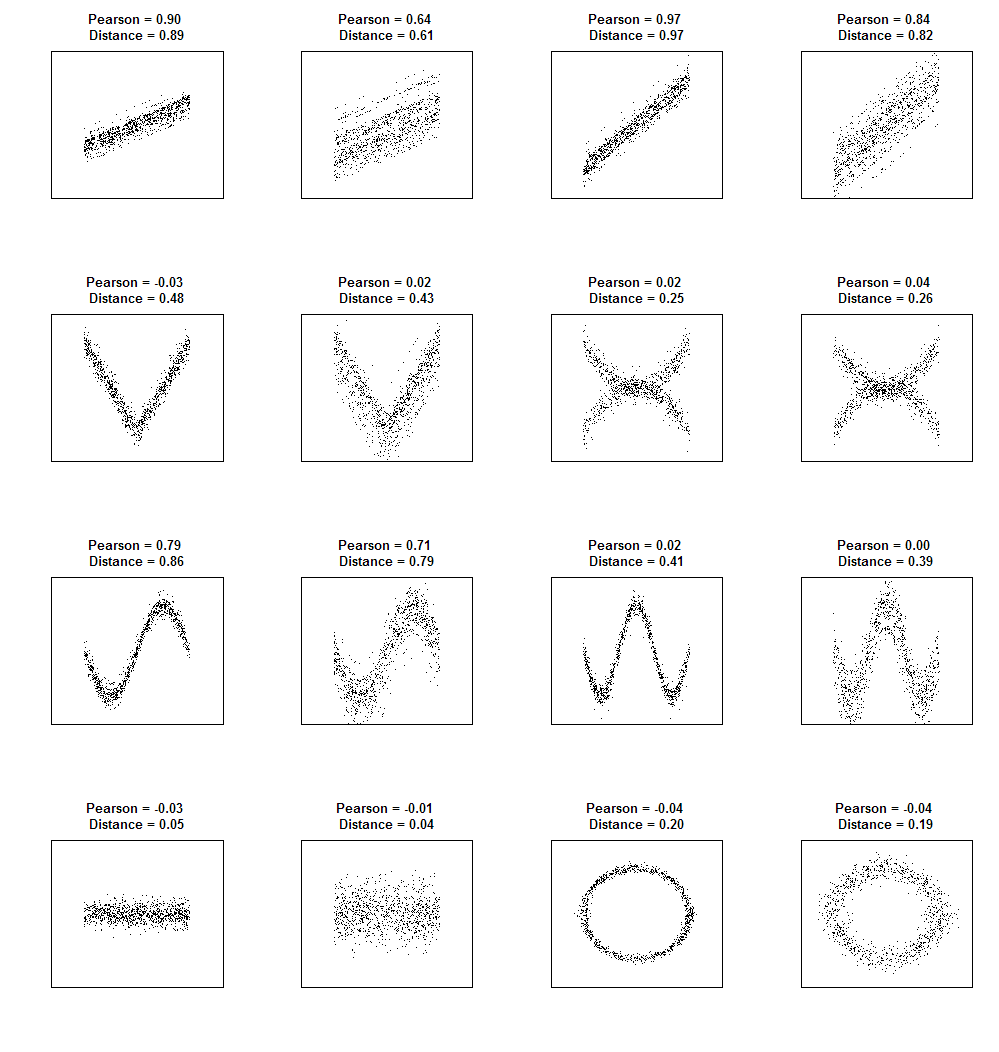
\includegraphics[scale = 0.8]{figs/1_nonlinear_depend.png}

Non-linear dependency relationships also exist in the ABIDE 50002 fMRI
data. The scatterplots below show time samples of spatially adjacent
voxels. These instances were found by searching for the maximum
difference in rank of energy distance correlation and the coefficient
of determination, or Pearson squared.

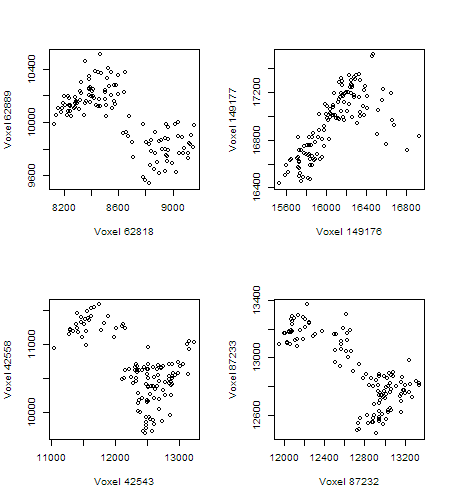
\includegraphics[scale = 0.7]{figs/1_nonlinear_ABIDE_50002.png}

Many studies on functional parcellation (Craddock 2012; Bellec 2006;
Heller 2006) use Pearson's coefficient as the similarity measure between
nearby voxels. Apart from underestimating the important of non-linear
relationships, this method also distinguishes positive, upward-sloping
correlation from negative. As a result in many of the edges between
different parcels, the corresponding voxels would be strongly dependent
with negative correlation.


\section{About the Data}
{\color{blue}

Autism spectrum disorders (ASD) represent a formidable challenge for
psychiatry and neuroscience because of their high prevalence, lifelong
nature, complexity and substantial heterogeneity. Roughly 1\% of
children worldwide are diagnosed with ASD \cite{centers2010autism}.
We approach the parcellation problem by using the Autism Brain Imaging
Data Exchange (ABIDE) -- a consortium aggregating and openly sharing
1112 existing resting-state functional magnetic resonance imaging
(R-fMRI) data sets with corresponding structural MRI and phenotypic
information from 539 individuals with ASDs and 573 age-matched typical
controls (TCs; 7–64 years).

For simplicity in this thesis, we focus on
\{NUMBER OF SUBJECTS YOU'RE ACTUALLY USING\}
scanned at the University of Pittsburgh School of Medicine.
These autistic subjects included individuals from 7 to 35 years of age,
with a well-characterized Autistic Disorder. The Autism Diagnostic
Interview-Revised \cite{lord1994autism} and the Autism Diagnostic
Observation Schedule-General \cite{lord2000autism}, as well as expert
clinical opinion, were used to diagnose autism. Typical controls were
healthy individuals, with no history of head trauma, birth
complications, seizures, or psychiatric disorder. TC matched
individually to the participants with autism on age (within 1.5 y in
children, 3.5 y in adults), full-scale IQ (within 12 points) and gender.
Individuals with Autistic Disorder were referred from the Center for
Excellence in Autism Research (CEFAR) and the Autism Center of
Excellence (ACE). TC were recruited from previous studies at the LNCD or
by fliers and announcements.
\{If you want to know, I got this information from
\url{http://fcon_1000.projects.nitrc.org/indi/abide/}.
You probably can include this url directly or something.\}

In order to register each subject's brain to a common brain space, we
use the Montreal Neurological Institute's standardized brain
\cite{evans19933d,collins1994automatic}.
The MNI wanted to define a brain that is more representative of the
population. They created a new template that was approximately matched
to the Talairach brain in a two-stage procedure. First, they took 241
normal MRI scans, and manually defined various landmarks, in order to
identify a line very similar to the AC-PC line, and the edges of the
brain. Each brain was scaled to match the landmarks to equivalent
positions on the Talairach atlas. They then took 305 normal MRI scans
(all right handed, 239 M, 66 F, age 23.4 +/- 4.1), and used an
automated 9 parameter linear algorithm to match the brains to the
average of the 241 brains that had been matched to the Talairach atlas.
From this they generated an average of 305 brain scans thus transformed
- the MNI305. The current standard MNI template is the ICBM152, which
is the average of 152 normal MRI scans  that have been matched to the
MNI305 using a 9 parameter affine transform. The International
Consortium for Brain Mapping adopted this, the MNI152, as their
standard template, and this is the template we will be using. We use
the unsymmetrical MRI scan from MNI152 corresponding to voxels
corresponding to cubes with an edge-length of 2 millimeters. This
MNI152 template are $91\times 109 \times 91$ voxels in dimension but
only 228,453 voxels represent the brain (25\% of the total volume).

We preprocessed the raw data from ABIDE using the Configurable Pipeline
for the Analysis of Connectomes (C-PAC) alpha version 0.3.9. C-PAC is
an open-source software pipeline for automated preprocessing and
analysis of resting-state fMRI data. The image preprocessing steps
included slice-timing and motion correction based on the Friston Model,
nuisance signal regression (including 5 CompCorr signals, the
cerebrospinal fluid (CSF), motion and the global, linear, and quadratic
signals) and temporal filtering (0.001-0.08Hz). The derived R-fMRI
measures were normalized to Montreal Neurological Institute (MNI152)
stereostatic space (2mm$^3$ isotropic) with linear regressions and
spatially smoothed (applied FWHM = 6mm).

We then converted the 4-dimensional fMRI data (i.e., a 3-dimensional
image varying with time) in a 2-dimensional matrix whereby each column
represents a different voxel and each row represents a different sample
from a different time. Since C-PAC removed most autocorrelations in the
data, we can reasonably treat each observation (i.e, each row) as drawn
from the same unknown distribution.
}

In this investigation, all parcellation and validation procedures were
conducted on the ABIDE 50002 fMRI data set. This data set contains
233305 voxels and 124 time samples. Spatial information is encoded as a
graph; each voxel is represented by a vertex, and each vertex has up to
6 edges connecting the voxel to its cubically adjacent neighbors. The
weights on the edges are sample energy distance correlations between the
two connected voxels (Szekely 2013).

\section{Notation}
{\color{red}If you don't have any, you can omit this section :p}

\section{Chapter Summaries}
{\color{red}Put the last part of what was currently in your abstract
here.}



\chapter{Energy Statistics}
%#######################################################################

In this Chapter, we present the theory of distance correlation and
justify its advantages over traditional statistics such as Pearson's
for brain parcellation. Distance correlation belongs to a family of
nonparametric statistics called energy statistics, which was first
developed by G\'{a}bor Sz\'{e}kely as a measure of dissimilarity between
probability distributions that formed the basis for nonparametric
goodness-of-fit tests. Subsequent results extended energy statistics
to problems of multivariate statistical dependence in
\cite{szekely2007measuring} and \cite{bakirov2006multivariate}.
Following this many applications of distance correlation and distance
covariance have been developed. A review of these can be found in
\cite{szekely2013energy}. Our exposition on energy statistics draws
primarily from this review.

Distance correlation is a non-linear measurement of statistical
dependency between two random variables of arbitrary dimension, and it
equals zero if and only if the two random variables are independent.
In our parcellation approach, we will compute the sample distance
correlation between each voxel and its 6 cubically adjacent neighbors
and set them as the weights of the corresponding edges. Then, edges
whose endpoints are in the same parcel can be used as a measure of the
statistical dependency between adjacent voxels in a parcel, and edges
whose endpoints lie in different parcels can be used to measure the
statistical dependency at parcel boundaries. Both our criteria for
measuring the goodness of a parcellation and the objective functions
that our algorithms seek to maximize depend on distance correlation
weights of the brain graph.

\section{Non-linear Dependencies in fMRI Data}

\begin{figure}
\caption{Pearson's and Distance Correlation for Linear and %
Non-linear Relationships}
\label{nonlinear_depend}
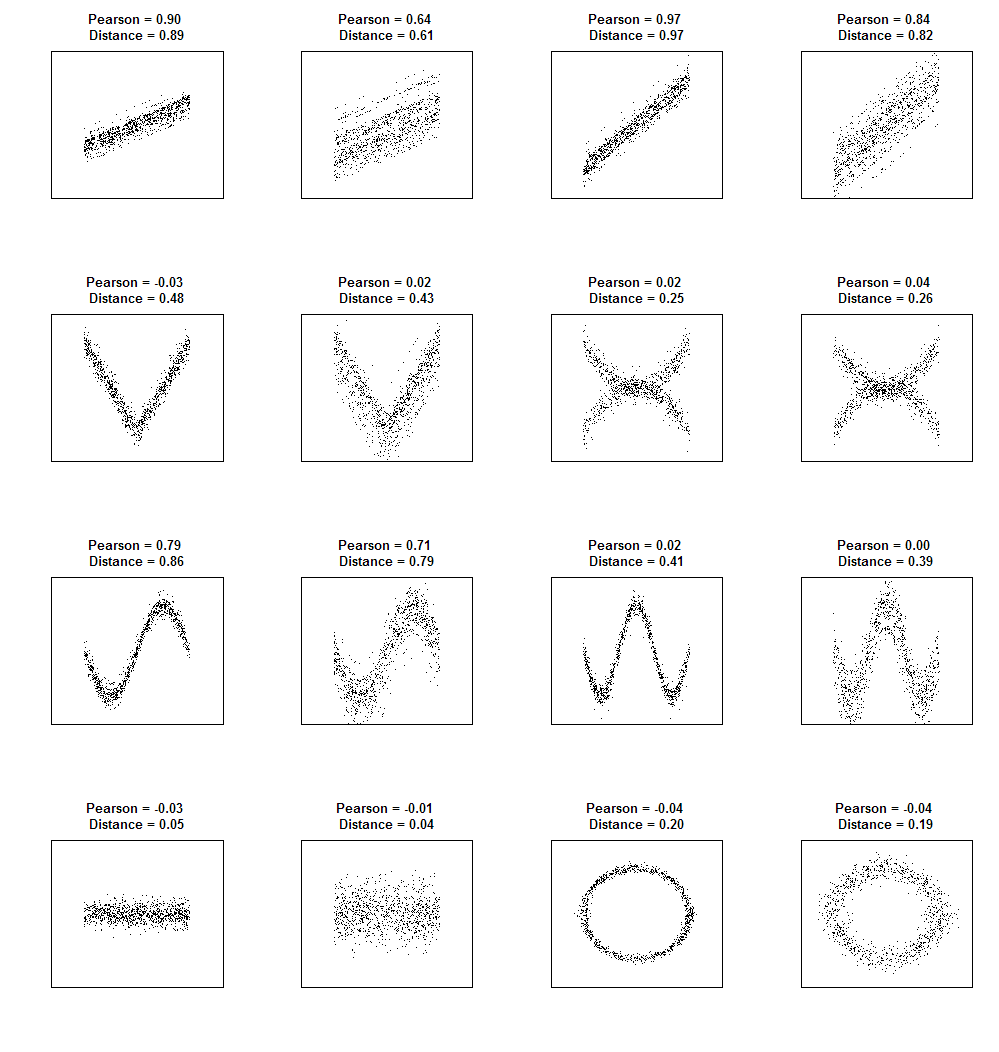
\includegraphics[scale = 0.8]{figs/1_nonlinear_depend.png}
\end{figure}

To measure dependence, statisticians have traditionally used Pearson's
correlation coefficient, in addition to the rank-based Kendall tau and
Spearman rho. These statistics work well when the underlying
relationship between the two random variables is already linear, in the
case of Pearson, or can be linear after a monotonic transformation, in
the case of Kendall and Spearman. Due to their restrictions, these
correlation coefficients will fail to capture many kinds of dependency
relationships. Figure \ref{nonlinear_depend} illustrates cases of
linear and non-linear relationships between random variables and their
sample Pearson and distance correlation values.

\begin{figure}
\caption{Four Instances of Strongly Non-Linear Relationships Between %
Adjacent Voxels in fMRI Data}
\label{fmri_nonlinear}
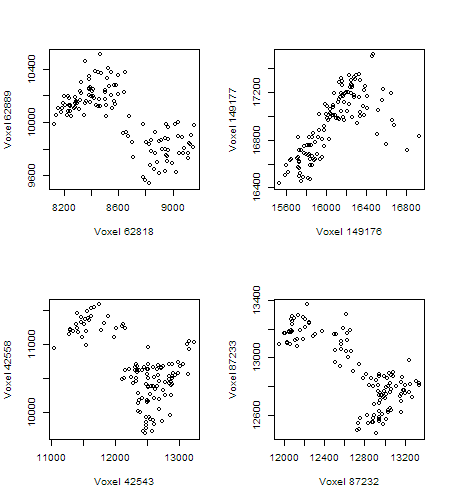
\includegraphics[scale = 0.7]{figs/1_nonlinear_ABIDE_50002.png}
\end{figure}

Non-linear dependency relationships also exist in the fMRI data. The
scatterplots in Figure \ref{fmri_nonlinear} show time samples of
spatially adjacent voxels with particularly strong non-linear
relationships.\footnote{These instances were found by searching for the
maximum difference in rank of energy distance correlation and the
coefficient of determination, or Pearson squared.} Hence using distance
correlation as the edge weights in the voxel graph has an obvious
advantage to using Pearson's correlation.

\section{Distance Covariance, Variance, and Correlation}

We first discuss the definition and properties of distance covariance,
from which the definition of distance correlation will naturally
follow. We first start with the population quantity where
$\mathcal{V}(X,Y)$ represents the population distance covariance
between two distributions, one over the random variable $X$ in a
$p$-dimensional space and the other over $Y$ in a $q$-dimensional
space.

Let $\varphi_X(s) = \Expect[e^{i s^T X}]$ denote the characteristic
function of a random vector $X$. For some positive weight function
$w : \R^p \times \R^q \mapsto [0, \infty)$ define the norm
$\|\cdot\|_w : \{\gamma : \R^p \times \R^q \mapsto \mathbb{C}\}
               \mapsto [0, \infty)$ as
\[ \|\gamma\|_w^2 = \int_{\R^{p+q}} |\gamma(s,t)|^2 w(s,t)
                    \diff s \diff t. \]

In the case where the subscript $w$ is omitted, it is implied that
$w(s,t) = 1$, the constant function taking value one. Hence
$\|\cdot\|^2$ is the typical definition of the $\ell_2$ (Euclidean)
norm squared.

\begin{definition}[Distance covariance] 
Let $X$ and $Y$ be two $p$ and $q$-dimensional (respectively) random
vectors with finite first moments and characteristic functions
$\varphi_X$ and $\varphi_Y$. Let the weight function
$w(s,t) = \dfrac{c_p c_q}{\|s\|^{1+p} \|t\|^{1+q}}$ where
$c_d = \dfrac{\Gamma(\frac{d+1}{2})}{\pi^{(d+1) / 2}}$
The \textit{squared} distance covariance between $X$ and $Y$ is defined
\begin{align*}
\mathcal{V}^2 (X,Y)
&= \| \varphi_{X,Y}(s,t) - \varphi_X(s)\varphi_Y(t) \|_w^2 \\
&= c_p c_q \int_{\R^{p+q}}
   \dfrac{|\varphi_{X,Y}(s,t) - \varphi_X(s)\varphi_Y(t)|^2}
         {\|s\|^{1+p} \|t\|^{1+q}} \diff s \diff t.
\end{align*}
Distance covariance is defined
$\mathcal{V}(X,Y) = \sqrt{\mathcal{V}^2(X,Y)}$.
\end{definition}

Distance covariance has the immediate property that
$\mathcal{V}(X,Y) = 0$ if and only if
$\varphi_{X,Y}(s,t) - \varphi_X(s) \varphi_Y(t) = 0$ for all
$s \in \R^p$ and $t \in \R^q$.

Random vectors $X$ and $Y$ are defined to be statistically independent
if and only if their joint density function $p_{X,Y}$ factors into the
product of the marginal densities of $X$ and $Y$. The one-to-one
correspondence between probability densities and characteristic
functions gives us the following:

\begin{theorem}[Kac's Theorem]
Let $X$ be $p$-dimensional and $Y$ $q$-dimensional random variables.
Then $X$ and $Y$ are independent if and only if for all $s \in \R^p$
and all $t \in \R^q$,
\[ \Expect[e^{i (s^T X + t^T Y)}]
 = \Expect[e^{i s^T X}] \Expect[e^{i t^T Y}] \]
\end{theorem}
\begin{proof}
($\implies$): If $X$ and $Y$ are independent, then
$\Expect[f(X) g(Y)] = \Expect[f(X)] \Expect[g(X)]$ for any functions
$f$ and $g$.

($\impliedby$): Let $\tilde{X}$ and $\tilde{Y}$ be independent
variables with the same marginal distribution as $X$ and $Y$. Then
\begin{align*}
\Expect[e^{i (s^T X + t^T Y)}]
&= \Expect[e^{i s^T X}] \Expect[e^{i t^T Y}] \\
&= \Expect[e^{i s^T \tilde{X}}] \Expect[e^{i t^T \tilde{Y}}] \\
&= \Expect[e^{i (s^T \tilde{X} + t^T \tilde{Y})}]
\end{align*}
The first equality comes from the premise, the second by the equal
distributions of $X$ and $\tilde{X}$, and the third by the independence
of $\tilde{X}$ and $\tilde{Y}$. Since the characteristic function
uniquely describes a distribution, $(X, Y)$ has the same joint
density function as $(\tilde{X}, \tilde{Y})$. Hence the joint density
of $X$ and $Y$ factorizes into the marginal densities.
\end{proof}

The important corrollary to this theorem is that $\mathcal{V}(X,Y) = 0$
if and only if $X$ and $Y$ are independent. Next, we define the
distance variance $\mathcal{V}(X)$

\begin{definition}
[Distance variance]
$$ \mathcal{V} (X) = \mathcal{V} (X,X) $$
\end{definition}

Analogously to the regular definitions of variance, covariance, and
correlation, the distance correlation $\mathcal{R}(X,Y)$ is

\begin{definition}
[Distance correlation]
\[ \mathcal{R} (X,Y) = \begin{cases}
  \frac{\mathcal{V}(X,Y)}{\sqrt{\mathcal{V}(X) \mathcal{V}(Y)}}
  & \text{if } \mathcal{V}(X) \mathcal{V}(Y) > 0 \\
  0 & \text{otherwise}
\end{cases} \]
\end{definition}

Distance covariance, variance, and correlation are estimated from an
independent identically distributed random sample
$\{(X_i, Y_i)\}_{i=1}^n$ by replacing the population characteristic
function with the empirical characteristic function:
\[ \widehat{\varphi}_X (t) = \frac{1}{n} \sum_{i=1}^n \exp(i t^T X_i) \]
Let $\mathcal{V}_n(X,Y)$ denote the sample distance covariance obtained
by this substitution. From \cite{szekely2007measuring} we get the
following closed-form formula for $\mathcal{V}_n(X,Y)$:

\begin{theorem}[\cite{szekely2007measuring} (Theorem 1)]
Let $\{(X_i, Y_i)\}_{i=1}^n$ be a random sample drawn iid. Define
the Euclidean distance matrices $a_{ij} = \|X_i - X_j\|$ and
$b_{ij} = \|Y_i - Y_j\|$ for $i,j$ from 1 to $n$. Define the centered
distance matrix entries
\[ A_{ij} = a_{ij} - \overline{a}_i - \overline{a}_j + \overline{a} \]
where $\overline{a}_i$ is the mean of the $i$th row (or column) of
matrix $a$ and $\overline{a}$ is the mean of all entries of $a$. Define
the centered matrix $B$ from $b$ analogously for all $i,j = 1, ..., n$.
Then,
\[ \mathcal{V}_n(X,Y) = \sqrt{\frac{1}{n^2}
                              \sum_{i,j=1}^n A_{ij} B_{ij}} \]
\end{theorem}

The sample distance variance and correlation are defined in terms of
sample distance covariance in exactly the same manner as the population
versions.

We now review some key properties that relate the sample distance
covariance to the population distance covariance that helps give
insight. We simply state the theorems and refer to the papers for
interested readers.

First, we relate the distance correlation to Pearson correlation.

\begin{definition} [$\alpha$-distance covariance] 
For $0 < \alpha < 2$
$$ \mathcal{V}_\alpha^2 (X,Y)
 = \frac{1}{C(p,\alpha) C(q,\alpha)}
   \int_{\R^{p+q}} \frac{|\varphi_{X,Y}(s,t) -
                          \varphi_X(s) \varphi_Y(t)|^2}
                        {\|s\|^{\alpha + p} \|t\|^{\alpha + q}} ds dt $$
\end{definition}

\begin{prop}[\cite{szekely2013energy} (Section 7.2)]
If $\Expect[\|X\|^\alpha] + \Expect[\|Y\|^\alpha] < \infty$ then
$$ \mathcal{V}_\alpha^2 (X,Y) = \Expect[ \|X - X'\|^\alpha \|Y - Y'\|^\alpha ] + \Expect \|X - X'\|^\alpha \Expect \|Y - Y'\|^\alpha - 2 \Expect[ \|X - X'\|^\alpha \|Y - Y''\|^\alpha ]$$

In particular, if $\alpha = 2$, $p = q = 1$, the distance correlation is 
the absolute value of Pearson's correlation coefficient.
\end{prop}

Next, we show statement ensuring consistency under the existence of the
first moments.

\begin{prop}[\cite{szekely2007measuring} (Corollary 1)]
If $\mathbb{E}(\|X\| +\|Y\|)< \infty$, then almost surely
\[
\lim_{n\rightarrow\infty}\widehat{\mathcal{R}}(X,Y) = \mathcal{R}(X,Y)
\]
\end{prop}

While we did not find a theorem explicitly stating the rate of 
convergence, the above theorem gives us satisfaction that if
$\mathcal{V}(X,Y)=0$ (meaning $X$ and $Y$ are independent), then as long 
as we have enough samples, $\widehat{\mathcal{V}}(X,Y) $ will approach
0. In our case, $n$ refers to the number of time samples which
typically range from $n=100$ to $n=200$.

We next show the asymptotic distribution of the sample distance
covariance under independence of $X$ and $Y$. While this is not used in
our work (as we do not apply the hypothesis test), this can inspire
future work where instead of computing the sample energy statistics
$\widehat{\mathcal{V}}(X,Y)$, we compute the $p$-value
under the null hypothesis $H_0: X \indep Y$.

To formulate the asymptotic distribution, we need additional notation.
Let $Q$ be a random variable where
\[ Q \overset{D}{=} \sum_{j=1}^{\infty}\lambda_j Z^2_j, \]
where $Z_j$ are independent, standard normal random variables and
$\{\lambda_j\}$'s are nonnegative constants dependent on the
characteristic functions on the joint distribution $(X,Y)$ such that
$\mathbb{E}[Q] = 1$. Here, we put the superscript $D$ to denote equality 
in distribution.

\begin{prop}[\cite{szekely2007measuring} (Corollary 2)]
If $\mathbb{E}(\|X\| +\|Y\|)< \infty$, then
\begin{itemize}
\item If $X$ and $Y$ are independent, then $n\widehat{\mathcal{V}}^2/S_2 \overset{D}{\rightarrow} Q$.
\item If $X$ and $Y$ are dependent, then $n\widehat{\mathcal{V}}^2/S_2 \overset{P}{\rightarrow} \infty$.
\end{itemize}
\end{prop}

Here, the superscript $D$ and $P$ denote convergence in distribution and
probability as $n$ goes to infinity. More explicit asymptotic
distributions are given in \cite{szekely2013energy} when $X$ and $Y$ are
Gaussian, but in general, bootstrapping procedures can be used to test
this hypothesis. Similar procedures can be derived on the distance
correlation.

In all our computations throughout our thesis, we use the \texttt{dcor}
function in the \texttt{energy} package to compute the distance
correlation efficiently.


\chapter{Criteria for Evaluating Parcellations}
In Chapter 1 we discussed our graphical approach to the brain
parcellation problem. We construct a weighted undirected graph where
each vertex corresponds with a voxel. The graph reflects the spatial
position of the voxels; it connects each vertex to the vertices
representing the voxel's six cubically adjacent neighbors.

The weights on these edges are sample distance correlation statistics
$\mathcal{R}_n(X,Y)$ between the adjacent voxels $X$ and $Y$ in the
time series of fMRI data. The properties of $\mathcal{R}$ are presented
more thoroughly in the preceding Chapter. The most relevant one is that
$0 \leq \mathcal{R}_n(X,Y) \leq 1$, with higher distance correlation
indicating a greater degree of statistical dependency.

Let $G(V, E)$ denote the voxel graph, its vertices, and its edges.
A valid $k$-fold partition $\mathcal{P}_k$ of the graph $G$ is a
collection of vertex subsets $(V_1, ..., V_k)$ satisfying the following:

\begin{enumerate}[1.]
\item
$V_i \neq \emptyset$ for all $V_i \in \mathcal{P}_k$

\item
$\bigcup\limits_{i=1}^k V_i = V$

\item
$V_i \cap V_j = \emptyset$ for all $V_i, V_j \in \mathcal{P}_k$

\item
$V_i$ is connected (i.e. for every two vertices in $V_i$, there is a
path between them) for all $V_i \in \mathcal{P}_k$
\end{enumerate}

In this chapter we will suggest various criteria for measuring the
goodness of parcellations and discuss their statistical and
computational advantages and drawbacks. Our notation will be as follows:
Let $\mathcal{R}_n(x,y)$ denote the sample distance correlation between
two voxels $x$ and $y$. For any two parcels $V, W \in \mathcal{P}_k$ we
will use $E_V$ to denote the set of edges with one endpoint in $V$ and
one endpoint not in $V$, and $E_{V,W}$ the set of edges with one
endpoint in $V$ and one in $W$.

\section{Within-Parcel Dependency}

Voxels in the same parcel are ideally highly dependent on one another in
the time series of fMRI data. To measure the degree of statistical
dependence within a parcel, we begin with the idea of computing the
sample distance correlation between \textit{all} pairs of voxels in the
same parcel. We'll call this criterion the \textit{Within-Score}.
A good parcellation will have a large Within-Score.

\begin{definition}[Within-Score] \label{within-score}
\[ \frac{1}{k} \sum_{V \in \mathcal{P}_k}
   \frac{1}{|V|^2} \sum_{x,y \in V} \mathcal{R}(x,y)
\]
\end{definition}

The Within-Score is non-spatial; it considers all pairs of voxels
equally regardless of whether they are adjacent. Consequently, it is a
good measure of how much the voxels within each parcel are dependent on
each other as a set. The disadvantage of this criterion is that it is
very expensive to compute. With over 200,000 voxels in an fMRI data set
we would potentially have to compute tens of billions of distance
correlation statistics, each of which takes time proportional to the
number of samples squared.

An alternative and far less expensive criterion that measures within-
parcel similarity works by counting distance correlations between
adjacent pairs of voxels.

\begin{definition}[Adjacent-Score] \label{adjacent-score}
\[ \frac{1}{k} \sum_{V \in \mathcal{P}_k}
   \frac{1}{|E_{V,V}|} \sum_{(x,y) \in E_{V,V}} \mathcal{R}(x,y)
\]
\end{definition}

Rather than treat parcels as sets with no spatial information, the
Adjacent-Score does the opposite by only considering the pairwise
dependency of adjacent voxels. For sparse graphs such as ours, the
number of distance correlation computations is proportional to the
number of vertices. In our cubically adjacent voxel graph, it is bounded
above by $6 |V|$. Both the Adjacent-Score and Within-Score are
between 0 and 1.

We define the Maximize Average Within-Edge (MAWE) for $k$ partitions
problem as the problem of finding a valid $k$-fold partition
$\mathcal{P}_k$ of $V$ so as to maximize the Adjacent-Score
(\ref{adjacent-score}). MAWE will serve as the general guideline for our
parcellation algorithms in later chapters. Hence we adopt the
Adjacent-Score as our primary metric for evaluating the goodness of
parcellations for capturing functional connectivity.

\section{Between-Parcel Dependency}

Another way of viewing parcellation quality is to look at how
dependent voxels belonging to different parcels are on each other. To
this end we define two criterion similar to the Within-Parcel criterion;
a non-spatial metric called the Between-Score and its spatial metric
the Boundary-Score. Contrary to the within parcel criteria presented
above, the goal now becomes to \textit{minimize} the criteria measuring
between-parcel dependency.

\begin{definition}[Between-Score] \label{between-score}
\[ \frac{1}{\binom{k}{2}} \sum_{V, W \in \mathcal{P}_k, V \neq W}
   \frac{1}{|V||W|} \sum_{x \in V, y \in W} \mathcal{R}(x,y)
\]
\end{definition}

\begin{definition}[Boundary-Score] \label{boundary-score}
\[ \frac{1}{\binom{k}{2}} \sum_{V, W \in \mathcal{P}_k, V \neq W}
   \frac{1}{|E_{V,W}|} \sum_{(x,y) \in E_{V,W}} \mathcal{R}(x,y)
\]
\end{definition}

Generally both of these quantities are more expensive to compute than
their Within-Parcel counterparts. Boundary-Score is easy enough to
compute for validation purposes, but does not convey much additional
information beyond what the Adjacency-Score does, in the sense that
the edges used in the computation of Adjacency-Score are the complement
of the edges used in the Boundary-Score.

The ability of distance correlation to generalize to pairs of random
vectors of arbitrary dimension gives us another way of computing
the dependency between two parcels. The Multivariate Between-Score
defined below treats parcels as random vectors and computes the distance
correlation at the parcel level rather than voxel level. The result is
a measure of non-spatial between-parcel similarity that is also
computationally feasible. For this reason we will use Multivariate
Between-Score as our primary measure of parcel dissimilarity.
Between-Score, Boundary-Score, and Multivariate Between-Score all
lie between 0 and 1.

\begin{definition}[Multivariate Between-Score]
\label{multi-between-score}
\[ \frac{1}{\binom{k}{2}} \sum_{V, W \in \mathcal{P}_k, V \neq W}
   \mathcal{R}(V, W)
\]
\end{definition}

Closely related to the Boundary-Score is the notion of a graph cut from
computer science. A \textit{cut} is the set of edges with endpoints
in different parcels. The \textit{cut weight} is the sum of weights of
all edges in the cut set and can be expressed as
\[ \frac{1}{2} \sum_{V \in \mathcal{P}_k}
   \sum_{x,y \in E_V} \mathcal{R}(x,y) \]
The \textit{ratio cut} defined below is a weighted version of the cut
weight
\[ \frac{1}{2} \sum_{V \in \mathcal{P}_k} \frac{1}{|V|}
   \sum_{x,y \in E_V} \mathcal{R}(x,y)
\]
Although we do not use these two criteria directly in evaluating
parcellations, we include them here because of their importance in
the graph partitioning literature. In particular, the ratio cut has
a close connection with spectral partitioning methods explored in
Chapter 5.

\section{Balance and Jaggedness}

The previous criteria are concerned solely with measuring functional
connectivity within and between parcels, without regard for the spatial
shape of the parcels.
Both anatomical and functional parcellations in the literature exhibit
some degree of parcel shape regularity. The number of voxels in each
parcel does not vary too much, and the surface of parcels tend to be
smooth. We quantify these two attributes with the following criteria:

\begin{definition}[Balance] \label{balance}
\[ \frac{1}{k} \frac{1}{\underset{V \in \mathcal{P}_k}{\max} |V|}
   \sum_{V \in \mathcal{P}_k} |V| \]
\end{definition}

The Balance-Score has a maximum value of 1 which occurs if and only if
all parcels are equally sized. It is bounded asymptotically below by 0
and approaches this number as $k$ increases and there is one huge
parcel and $k - 1$ miniscule ones. In the Automatic Anatomical
Parcellation, the Balance-Score is around $0.3$. Our parcellations will
aim for around this number.

\begin{definition}[Jaggedness] \label{jaggedness}
\[ \frac{1}{k} \sum_{V \in \mathcal{P}_k} \frac{|E_V|^\frac{3}{2}}{|V|}
\]
\end{definition}

The Jaggedness criterion is a normalized graphical version of the mean
surface area to volume ratio of all parcels. The surface area here is
the number (not weight) of edges with only one endpoint in a parcel and
the volume is the number of vertices in the parcel.

The Jaggedness criterion is \textit{normalized} in the sense that the
$\frac{3}{2}$ power in the numerator makes the ``dimensionality'' of the
surface area (which is 2-D in the 3-D space) equal to dimensionality of
the volume (which is 3-D). This has the benefit of making the
surface-area to volume ratio not depend on the size of the parcel.
For instance, a $n \times n \times n$ cube of vertices would have
a jaggedness of $6^{\frac{3}{2}}$ which does not depend on $n$.

\section{Comparing Multiple Parcellations}

Since we'll be running our parcellation methods on multiple brains we
require a criterion that compares the similarity of two different
parcellations. We will be using the Adjusted Rand Index, which is a
common measure used in the clustering literature.

\begin{definition}[Adjusted Rand Index] \label{ari}
Let $\mathcal{P}_k = \{V_1, ..., V_k\}$ and
    $\mathcal{Q}_l = \{W_1, ..., W_l\}$ be two partitionings of $V$.
Let the overlap of $V_i$ and $W_j$ be denoted 
\[ n_{ij} = | V_i \cap W_j | \]
and let $a_i = \sum_{j=1}^l n_{ij}$ be the row sums and
        $b_j = \sum_{i=1}^k n_{ij}$ be the column sums of $[n_{ij}]$.
The Adjusted Rand Index (ARI) is defined as
\[ \frac{\sum_{i,j} \binom{n_{ij}}{2} -
         \frac{S}{\binom{n}{2}} 
        }
        {\frac{S}{2} - \frac{S}{\binom{n}{2}}} \]
where $S = \sum_i \binom{a_i}{2} + \sum_j \binom{b_j}{2}$
\end{definition}

The advantage of ARI is that the number of parcels in the two
parcellations compared do not have to be equal. The ARI has a value of
1 if and only if the two parcellations assign the same voxels to each
parcel. ARI values close to 0 indicate that parcellations are
independent of each other for any number of parcels, which would occur
if one of the two parcellations were randomly generated. It is possible
to get negative ARI values.


\chapter{Local Search and Graph Growing Heuristics}
% 1. in union-find subsection make function names in text a different
%    font
% 2. include parameters of size-constrained add-edge on randomized graph
%    in table
% 3. more analysis of SC AE results
%#######################################################################

We introduce several algorithms for generating brain parcellations. The
algorithms in this chapter are all local search heuristics; they begin
with $n$ unconnected vertices and iteratively join adjacent ones into
components until some stopping criterion is met.

For each algorithm, the resulting parcellation is presented, discussed,
and evaluated according to the criteria introduced in the previous
chapter.

\section{Unconstrained Add-Edge}

The first and simplest algorithm starts with an empty graph of $n$
vertices and sequentially adds edges between adjacent voxels in order of
highest sample distance correlation, until the graph has some
prespecified number of connected components $k$.

We will refer to this algorithm as ``Unconstrained Add-Edge''. A naive
implementation of would re-compute the number of connected components in
the graph (using linear-time bread-first or depth-first search) after
each addition of an edge, resulting in a costly $O(EN)$ time complexity.
A more efficient implementation takes advantage of the fact that each
addition of an edge decreases the number of components in the graph by
at most 1. Hence the algorithm needs only to compute the number of
connected components after adding $c - k$ edges, where $c$ is the
current number of connected components of the graph, beginning at $n$.

Another implementation uses a binary search-type strategy and is
$O((n + E) \log E)$. The idea is to ``search'' for the last edge to add
to the graph by maintaining a range of possible last edges. In each
iteration, the algorithm would add to the graph edges 1 to the midpoint
of this range, compute the number of connected components, and adjust
the range based on whether the number of components is higher or lower
than the target $K$.

The Unconstrained Add-Edge algorithm produces severely imbalanced
parcellations. In the 100-component graph, there was one component
containing over 99.9\% of all the vertices in the graph. This leads
to a modification that prevents some edges from being added when a
size constraint is violated.

\section{Size-Constrained Add-Edge}

The Size-Constrained Add-Edge algorithm works in a similar manner to the
unconstrained version, adding edges to the graph in decreasing order of
distance correlation. The Size-Constrained version differs by applying
a filter to each edge considered, adding the edge only if at least one
of the two following conditions are met:

\begin{enumerate}[1.]
\item
At least one of the two components bridge by the edge is of size less
than some prespecified parameter $s_{\min}$.

\item
The union of the two components is of size $\leq s_{\max}$.
\end{enumerate}

The restriction on adding new edges was not successful in creating
balanced partitions. For sake of completeness, we documented our
implementation.

The naive implementation must use BFS/DFS in each iteration to compute
the sizes of the two components to be connected by an edge, and hence
must have time complexity $O(EN)$. Fortunately, there is a way to
sublinearly update information on the components of the graph, using
the union-find data structure.

\subsection{Union-Find}

The core Union-Find data structure begins with an empty graph of $N$
vertices and supports two operations. union(i, j) adds an edge between
vertices $i$ and $j$. root(i) returns an identifier for the component
to which vertex $i$ belongs. All vertices in the same component have the
same root. We modified Union-Find to support an additional operation.
component\_size(i) returns the number of vertices belonging to the
component containing $i$.

Union-Find represents each component as a rooted tree, with vertices in
the graph mapping to nodes in the tree. Information about the tree is
stored in two arrays of length $N$, parent and size, which are subject
to the following invariants.

\begin{enumerate}[1.]
\item
For each node i, parent[i] = node i's parent on the tree, unless i is a
root node. If i is a root node, then parent[i] = i.

\item
Nodes i and j are in the same component if and only if they are in the
same tree, if and only if they share the same root node.

\item
If i is a root node, then size[i] = the size of the component, or the
number of nodes in the tree. If i is not a root node, then size[i] can
be anything.
\end{enumerate}

A baseline implementation of the three functions is

\begin{algorithm}
\caption{Union-Find}
\begin{algorithmic}

\Function{root}{i}
    \While{parent[i] $\neq$ i}
        \State i $\gets$ parent[i]
    \EndWhile
    \State \Return i
\EndFunction
\State 

\Function{union}{i, j}
    \State parent[root(j)] $\gets$ root(i)
\EndFunction
\State 

\Function{component\_size}{i}
    \State \Return size[root(i)]
\EndFunction

\end{algorithmic}
\end{algorithm}

In addition to the baseline code above, there are two important
optimizations:

\begin{enumerate}[1.]
\item
Weighted union maintains information of the sizes of each component so
that the root of the smaller component always becomes a child of the
larger component's root.

\item
Path compression flattens the tree with each call to root. Specifically,
when root is called on node $i$, each node traversed from $i$ to the
root has its parent set to be the root.
\end{enumerate}

With these two optimizations, the time complexity of root, union, and
component\_size has been shown to be at least as good as $O(\log^* N)$
where $\log^*$ is the iterated logarithm, defined as the number of
times the natural log must be applied to $N$ so that it becomes less
than or equal to 1.

\section{The Contractible Graph Data Structure and
Edge-Contraction Algorithm}

We propose a new data structure called the \textit{Contractible Graph}
(CG) for brain parcellation. The rationale behind the CG is a heuristic
procedure for partitioning a graph into somewhat balanced components
so as to maximize the Adjacent-Score (\ref{adjacent-score}).

The CG is a mapping of the vertices of the original graph to the
vertices of a new graph. The vertices of the CG are called
\textit{components} and between any two components there exists exactly
one weighted edge, henceforth called a \textit{link}. The weight
of a link $w_{A,B}$ between two components $A$ and $B$ in the CG equals
the average weight of all edges in the original graph between vertices
mapped to $A$ and vertices mapped to $B$. If no such edges exist,
the weight of the link is $0$. Formally,

\[ E_{A,B} = \{(i, j) \in E : i \in A, j \in B\} \]
\[ w_{A,B} = \begin{cases}
    \frac{1}{|E_{A,B}|} \sum_{(i,j) \in E_{A,B}} w_{ij} &
        \text{if } |E_{A,B}| > 0 \\
    0 & \text{otherwise}
\end{cases} \]

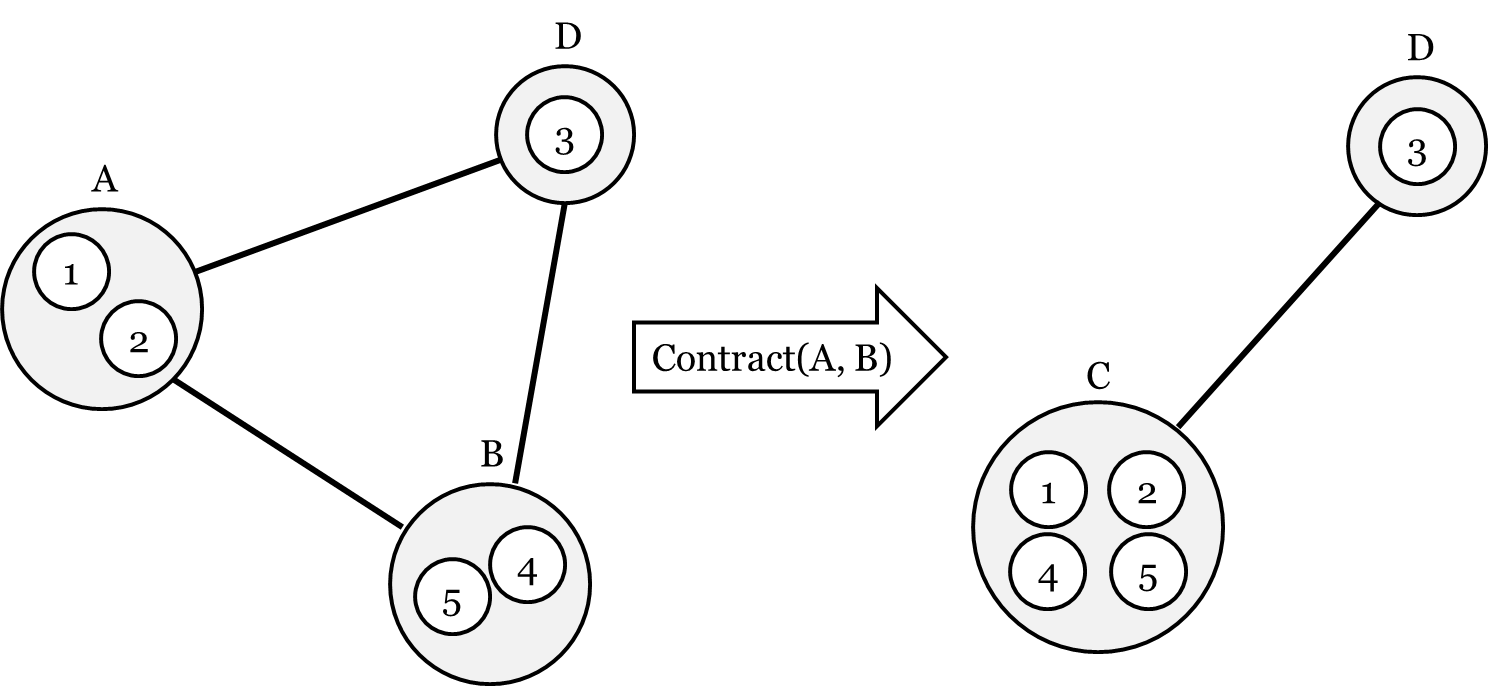
\includegraphics[scale = 0.5]{4_contractible_graph}

We say an edge $(i,j)$ is \textit{between} components $A$ and $B$ if
$i$ is in one of $A$ or $B$ and $j$ is in the other. The \textit{size}
of a component is the number of vertices it contains.
A \textit{contraction} of a link $(A,B)$ in a CG replaces components
$A$ and $B$ with a new component (call it $C$) containing all vertices
mapped to $A$ or $B$, as illustrated in the figure above.
Component $C$ has one link to every other component in the CG, whose
weights are the mean of the weights of the corresponding vertex edges,
or $0$ if no edge exists. Thus the contraction operation maintains the
link-invariant property of CG. This leads to the Edge-Contraction
algorithm, which begins with the original graph with all vertices as
singleton components and contracts edges in a certain order until the
graph has only $k$ components in all.

\begin{algorithm}
\caption{Edge-Contraction}
\begin{algorithmic}
\State \textbf{Input:} Undirected positive-weighted graph $G$ and
       target component number $k$
\State Create a CG from $G$ so that every vertex maps to
       a unique component
\Repeat
\State $\mathcal{S} \gets$ smallest component(s) in the CG
\State $(A,B) \gets \argmax{A \in \mathcal{S}} w(A,B)$
\State Contract $(A,B)$
\Until{CG has $k$ components}
\State \textbf{Output:} Components of CG
\end{algorithmic}
\end{algorithm}

Why does Edge-Contraction work better than the previous algorithms?
The Edge-Contraction algorithm attempts to address two problems of
the Size-Constrained Add-Edge algorithm: poor Adjacent-Score relative
to randomized graph and unbalanced parcels. We hypothesized that one
reason for a relatively low Adjacent-Score might be the following
scenario: when a vertex is added to a component, it might have multiple
edges to that component. One edge might have a very high weight; this is
the one that is officially ``added''. However, the other edges with far
lower weights are implicitly added as well, lowering the average edge
weights within the component.

The Edge-Contraction algorithm handles this issue by maintaining that
there can be at most one edge between any two components A and B, and
further that the weight on such an edge is the mean of the weights on
all edges that connect a vertex in A with a vertex in B.

\subsection{Implementation using Nested Hash Tables and Priority Queue}

In a Contractible Graph, the weight of the link between two components
depends on the summed weight of all edges between them, and the number
of such edges.

Our implementation of the CG uses \textit{nested hash tables},
diagrammed below. The outer hash table maps each component $A$ to an
inner hash table, which maps all components $B$ with a positive link to
$A$ to 1) the summed weights of the edges and 2) the number of edges
between $A$ and $B$.

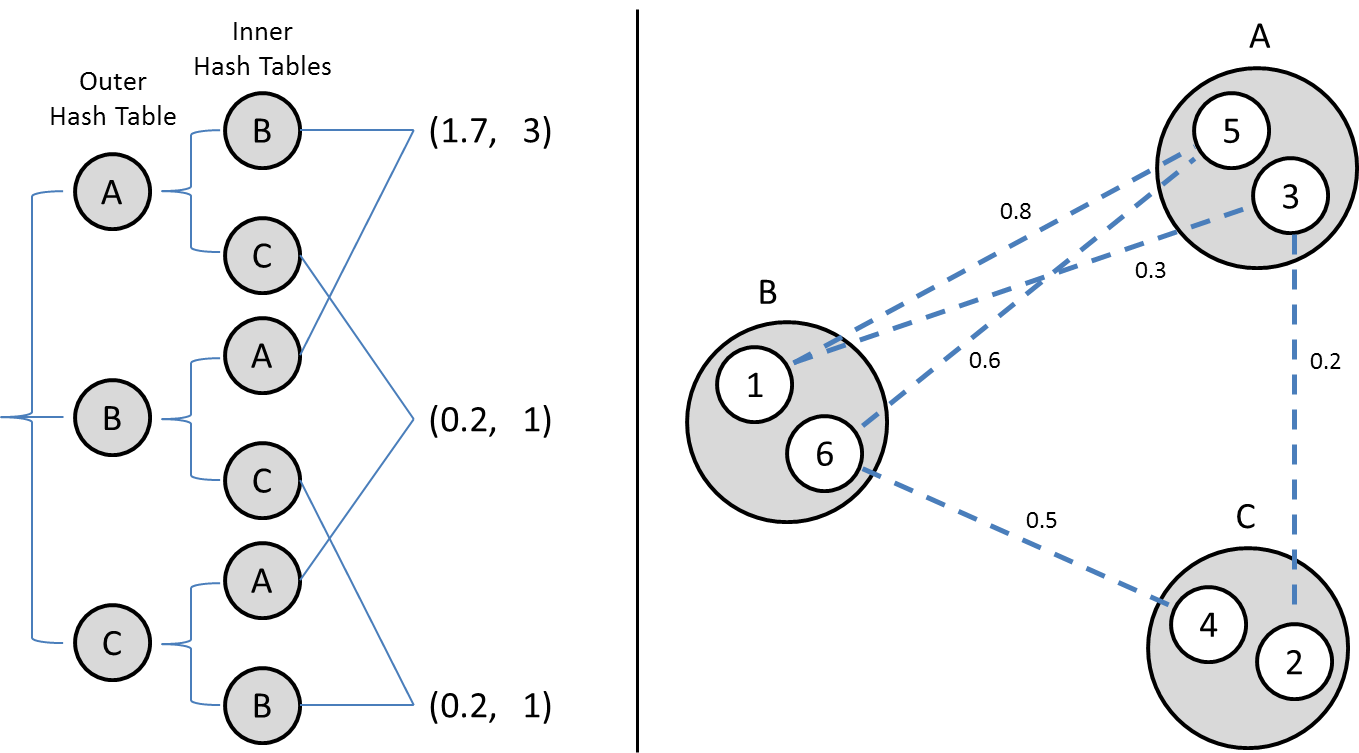
\includegraphics[scale = 0.5]{4_cg_implement}

Implementing the contraction of components $B$ and $C$ into a new
component $D$ on this nested hash table requires the following steps.
The time complexity is stated assuming no hash collisions.

\begin{enumerate}
\item
Compute $\mathcal{X}$, the set of all components that either $B$ or $C$
is linked to. $O(|E_B| + |E_C|)$

\item
Create a new element in the outer hash table, $D$, and associate it
with an empty inner hash table. $O(1)$

\item
For each component $X \in \mathcal{X}$,
\begin{itemize}
\item
Retrieve $W(X,B) + W(X,C)$, the summed weights all edges between $X$
and $B$ and between $X$ and $C$, and $|E_{X,B}| + |E_{X,C}|$, the
number of such edges. These quantities are stored explicitly as a
values in the inner hash table, so this operations is $O(1)$.

\item
Add a new component name $D$ to the inner hash table of $X$ and map it
to $\big( W(X,B) + W(X,C), |E_{X,B}| + |E_{X,C}| \big)$. Delete
elements $B$ and $C$ from the inner list of $X$. $O(1)$

\item
In the $D$ inner hash table, add component name $X$ and map it to
to the same $\big( W(X,B) + W(X,C), |E_{X,B}| + |E_{X,C}| \big)$.
$O(1)$
\end{itemize}

\item
Delete $B$ and $C$ from the outer list.
\end{enumerate}

Having described the contraction step, we will next discuss how to
efficiently locate the link to be contracted.
In computer science, a \textit{Maximum Priority Queue} (MaxPQ) data
type is a set of well-ordered objects that supports the following
operations:

\begin{itemize}
\item
\textit{add(obj)}: Adds an object to the set.

\item
\textit{remove\_maximum()}: Removes and returns an object with the
largest priority in the set.
\end{itemize}

Using the heap data structure, the above two operations both run in
$O(\log n)$ time.

Each component on the CG will be associated with an element of the
priority queue. The priority of component $A$ is defined as
\[ \max_{X}\;w_{A,X} - |A| \]
Since our graph link and edge weights are all between 0 and 1, the
highest priority element in the queue always has the smallest size.
Therefore, if the priority queue is up-to-date with the CG, the
next link to be contracted according to Edge-Contraction has
an endpoint component whose priority is the highest in the queue.

However, a complication arises from the fact that a contraction can
change the priorities of components neighboring the contracting
components, thereby making the priorities stored in the MaxPQ
out-of-date. For instance, if components $A$ and $B$ are contracted, and
there is a component $C$ with positive links to both $A$ and $B$, then
the $C-A$ and $C-B$ links will be replaced by a $C-(AB)$ link with a
different weight. If either $C-A$ or $C-B$ links happened to be the
maximum-weighted links of $C$, then $C$'s priority will be lower,
and $C$ ought to be further down the queue.

To address this issue, we could re-compute the priority of every
component drawn from the MaxPQ. If the component's actual priority is
not the maximum, then it is re-inserted into the queue with updated
priority. Additionally, the maximum priority component may no longer
exist in the CG due to contraction with another component. In this case
it is simply discarded.

Without using an efficient priority queue, the linear searching method
of finding the next link to contract results in a $O\big(n (n-k)\big)$
time algorithm. Using the priority queue the time complexity of
Edge-Contraction is $O \big((n - k) (m + \log n)\big)$, where $m$ is
the average number of positive links a component has.

\subsection{Results and Extensions}

\begin{figure}
\caption{Results of Edge-Contract for Different Component Numbers}
\csvautotabular{4_edge_contract_results.csv}
\end{figure}

The Edge-Contract parcellations notably outperformed the anatomical AAL
parcellation in the Adjacency-Score. For further comparison, found the
mean edge weight in the graph to be 0.7258, which is even slightly
higher than the average adjacent within-parcel edge in AAL. This suggests
that the AAL parcellation has no connection with the functional
information contained in this fMRI data set. It shows on the other
hand that the Edge-Contract algorithm can successfully locate regions of
functional similarity.

The one apparent deficiency of Edge-Contract is the jaggedness of its
parcels. Comparison of our parcellations with the AAL shows that our
116-component parcellation -- the same number of components as AAL --
has an average parcel surface area roughly
$\big( \frac{92.14}{29.62} \big)^{\frac{2}{3} }\approx 2.11$ times
that of AAL. Visually, that difference is shown in the plots below of
a typical component from each parcellation.

%\includegraphics[scale = 1]{4_edgecontract_aal_3D}

\section{Generalized Edge-Contraction}

In the original Edge-Contraction algorithm, the criteria for selecting
the next link to contract was to search through the set of smallest
components and find the link of maximal weight. Because this criteria
takes no account of the shape of the two components to be contracted,
the resulting parcels tend to be very jagged.

To address this we expanded the criterion for finding the next link
to contract. Rather than use only the size of the component and the
weight of the link, a \textit{Generalized Edge-Contraction} algorithm
may use any piece of information stored in the Contractible Graph about
a pair of components, such as the number of edges connecting two
components. A \textit{priority function} takes information of any two
components in a CG and outputs a real number, the priority. For each
iteration, the pair of components with the largest priority is
contracted and the priorities of neighboring components with respect
to the newly conjoined component are computed.

For two components $A,B$ let $|A|$ denote size (number of vertices)
of $A$, $E_{A,B}$ denote the set of edges between $A$ and $B$, and
$w_{A,B}$ the weight of the link connecting $A$ and $B$.
The priority function of the original Edge-Contraction algorithm
is $p_0(A, B) = w_{A,B} - |B|$.

A link $(A, B)$ will have high priority if either component is small,
if the link has a large weight, and if it has a good boundary-ratio,
defined as $\frac{|E_{A,B}|}{\min(|A|,|B|)}$, which helps to minimize
jaggedness. From these notions we created a family of priority functions indexed by tunable parameters $\alpha$ and $\beta$
\[ p_1(A, B) = \frac{w_{A,B}^\alpha}{|A| + \beta}
               \frac{|E_{A,B}|}{\min(|A|,|B|)} \]
that modulate the balance of small size, large weight, and high
boundary ratio. The table below shows the results of the 116-component
and 300-component Generalized Edge-Contract parcellation when performed
for various values of $\alpha$ and $\beta$.

\begin{figure}
\caption{Results of Generalized Edge-Contract for Various Parameter Settings}
%\csvautotabular{4_gen_edge_contract_results.csv}
\end{figure}




\chapter{Spectral Methods}
% Need to fix optimization problems -- add spacing between min and obj
%#######################################################################

In the previous chapter, we showed how local search heuristics produced
parcels that were balanced and had high within-parcel and low
between-parcel edge weights. The central idea behind such methods
was to choose vertices to be in the same component if the edge
connecting them has high distance correlation. Vertices were added to
components one-by-one with constraints on component size, but not on
component shape. As a result, one salient issue with these
parcellations was lack of smoothness, or regularity in the parcels'
spatial shapes. There was scant resemblence between the anatomical maps
of the brain depicting smooth, rotund lobes and our jagged, web-like
parcellations.

One key reason for this phenomenon are the local search heuristics'
focus on maximizing \textit{average} within-component edge weights
(equivalently, minimizing \textit{average} between-component edge
weights because edges are either within the same component or between
different components). To get smoothness in the boundary between
components, we could either impose a penalty for too many
between-component edges and work that into the local search heuristics,
or try minimizing over the sum of all weights on between-component
edges. This chapter deals with the second approach and this family of
methods is called spectral partitioning.

Spectral partitioning constitutes the second major class of techniques
used to partition graphs. Rather than rely on local component-growing
heuristics, spectral partitioning uses information about the entire
graph at once.

Throughout this chapter, a valid partitioning
$P_k = (V_1, ..., V_k)$ of the graph $G = (V, E)$ is defined in the
same way as in chapter 3; i.e., it must satisfy

\begin{enumerate}[1.]
\item
$V_i \neq \emptyset$ for all $V_i \in \mathcal{P}_k$

\item
$\bigcup\limits_{i=1}^k V_i = V$

\item
$V_i \cap V_j = \emptyset$ for all $V_i, V_j \in \mathcal{P}_k$

\item
$V_i$ is connected (i.e. for every two vertices in $V_i$, there is a
path between them) for all $V_i \in \mathcal{P}_k$
\end{enumerate}

For all edges $(i,j) \in E$, let $w_{ij}$ denote the weight of the edge
connecting vertices $i$ and $j$.
$S^{n \times n}$ is the set of real symmetric $n \times n$ matrices.
We further define, for a given graph $G = (V, E)$, the associated

\begin{definition}
Adjacency matrix. $A \in \mathcal{S}^{n \times n}$ has entries
\[
A_{ij} = \begin{cases}
  w_{ij} & \text{if } (i,j) \in E \\
  0      & \text{otherwise} \\
\end{cases}
\]
\end{definition}

\begin{definition}
Degree matrix. $D \in \mathcal{S}^{n \times n}$
\[
D_{ij} = \begin{cases}
  \sum_{k = 1}^n A_{ik} & \text{if } i = j \\
  0                     & \text{otherwise} \\
\end{cases}
\]
\end{definition}

\section{Size-Constrained MinCut and Graph Bipartitioning}

Consider the case $k = 2$. For all $i \in V$, let $x_i = 1$ if
$i \in V_1$ and $x_1 = -1$ if $i \in V_2$. Then the sum of weights on
edges between the two components is
\begin{align*}
C(P_2)
&= \sum_{i \in V_1} \sum_{j \in V_2} A_{ij} \\
&= \sum_{i = 2}^n \sum_{j = 1}^{i-1} \frac{(x_i - x_j)^2}{4} A_{ij} 
\end{align*}
since
\[ (x_i - x_j)^2 = \begin{cases}
	4 & \mbox{if } i,j \mbox{ are in different components} \\
	0 & \mbox{otherwise}
\end{cases}\]

$C(P_2)$ can also be written in a matrix quadratic form, as

\begin{align*}
C(P_2)
&= \sum_{i = 2}^n \sum_{j = 1}^{i-1} \frac{(x_i - x_j)^2}{4} A_{ij} \\
&= \frac{1}{2} \sum_{i,j = 1}^n \frac{(x_i - x_j)^2}{4} A_{ij} \\
&= \frac{1}{2} \sum_{i,j = 1}^n
   \frac{x_i^2 + x_j^2 - 2 x_i x_j}{4} A_{ij} \\
&= \frac{1}{2} \sum_{i,j = 1}^n \frac{1 - x_i x_j}{2} A_{ij} \\
&= \frac{1}{4} \sum_{i,j = 1}^n (x_i^2 - x_i x_j) A_{ij} \\
&= \frac{1}{4} \sum_{i = 1}^n x_i^2 \sum_{j = 1}^n A_{ij}
 - \frac{1}{4} \sum_{i,j = 1}^n x_i A_{ij} x_j \\
&= \frac{1}{4} \sum_{i = 1}^n x_i^2 D_{ii} - \frac{1}{4} x^T A x \\
&= \frac{1}{4} x^T (D - A) x \\
&= \frac{1}{4} x^T L x
\end{align*}
where $L$ is called the Laplacian matrix of the graph and defined as
$L = D - A$. MinCut can thus be formulated as minimizing $x^T L x$
subject to $x \in \{-1, 1\}^n$.

Algorithms like Karger's can solve MinCut in polynomial time. However,
MinCut in this formulation lacks constraints on the size of the
partitions, and if applied to our brain parcellation problem, would
result in severely inbalanced partitions. If constraints on the sizes
of the components were added, the problem becomes NP-hard [citation].

An old but effective approach to bipartitioning uses the eigenvectors
of the Laplacian matrix and is called spectral bipartitioning.
The approach relaxes the $\{-1, 1\}$ constraint on $x$ (and rescales
$x$) so that it need only satisfy $\|x\| = 1$ ($\|\cdot\|$ here refering
to L2 norm). It is easy to see that
$\big\{ x : x \in \{-\frac{1}{\sqrt{n}}, \frac{1}{\sqrt{n}}\}^n \big\}
 \subset \big\{ x \in \R^n : \|x\| = 1 \big\}$
The problem now becomes

\begin{equation} \label{spectral_bipartition}
\begin{aligned}
\min_x      &\;& x^T L x \\
\text{s.t.} &\;& \| x \| = 1 \\
\end{aligned}
\end{equation}

Using Lagrangian multipliers, it can be shown that all optimal solutions
to the above must satisfy $L x = \lambda x$ and this problem reduces to
finding the smallest eigenvalues of $L$ and their associated
eigenvectors. In addition, \ref{Laplacian_psd} below implies that all
eigenvalues are nonnegative.

\begin{theorem} \label{Laplacian_psd}
Let $L$ be a Laplacian matrix. Then $L \succeq 0$
($L$ is positive semidefinite)

Proof. Let $x \in \R^n$. $x^T L x = x^T D x - $
\end{theorem}

Note that from the
$C(P_2) = \sum_{i > j} \frac{(x_i - x_j)^2}{4} A_{ij}
        = \frac{1}{4} x^T L x$ equivalence we know that
$0$ and $(\frac{1}{\sqrt{n}}, ..., \frac{1}{\sqrt{n}})^T$ is a minimum
eigenvalue and eigenvector to this system. For bipartitioning, the
useful eigenvector is the one that corresponds to the 2nd smallest
eigenvalue, which is nonzero if the graph as a whole is connected.
We'll denote this eigenvalue as $\lambda_1$ and corresponding unit
eigenvector as $x_1$. We have the following:

\begin{theorem}
Let $P_2$ be any valid partition into 2 components. Then
$C(P_2) \geq \lambda_1$

Proof.
\end{theorem}

In the literature, $x_1$ is often refered to as the Fiedler vector,
after the first mathematician who studied it in detail [Fiedler 1975].
From the Fiedler vector we can obtain a variety of "good" bipartitions.
We can impose a size constraint $|V_1| = s$ and obtain a bipartition
satisfying this by placing the vertices associated with the $s$ largest
entries of $x_1$ in $V_1$. This encompasses bipartitions of equal
component size. We can also sort the entries of $x_1$ and find the
largest difference between consecutive sorted entries. Vertices
corresponding to entries sorted to the left of this split can be placed
in $V_1$ and vertices sorted to the right in $V_2$. This method tends to
approximate the MinCut solution.

The result of spectral bipartitioning on a resting state fMRI scan
is shown below. As anticipated, the boundaries of between the
components are smooth.

\begin{center}
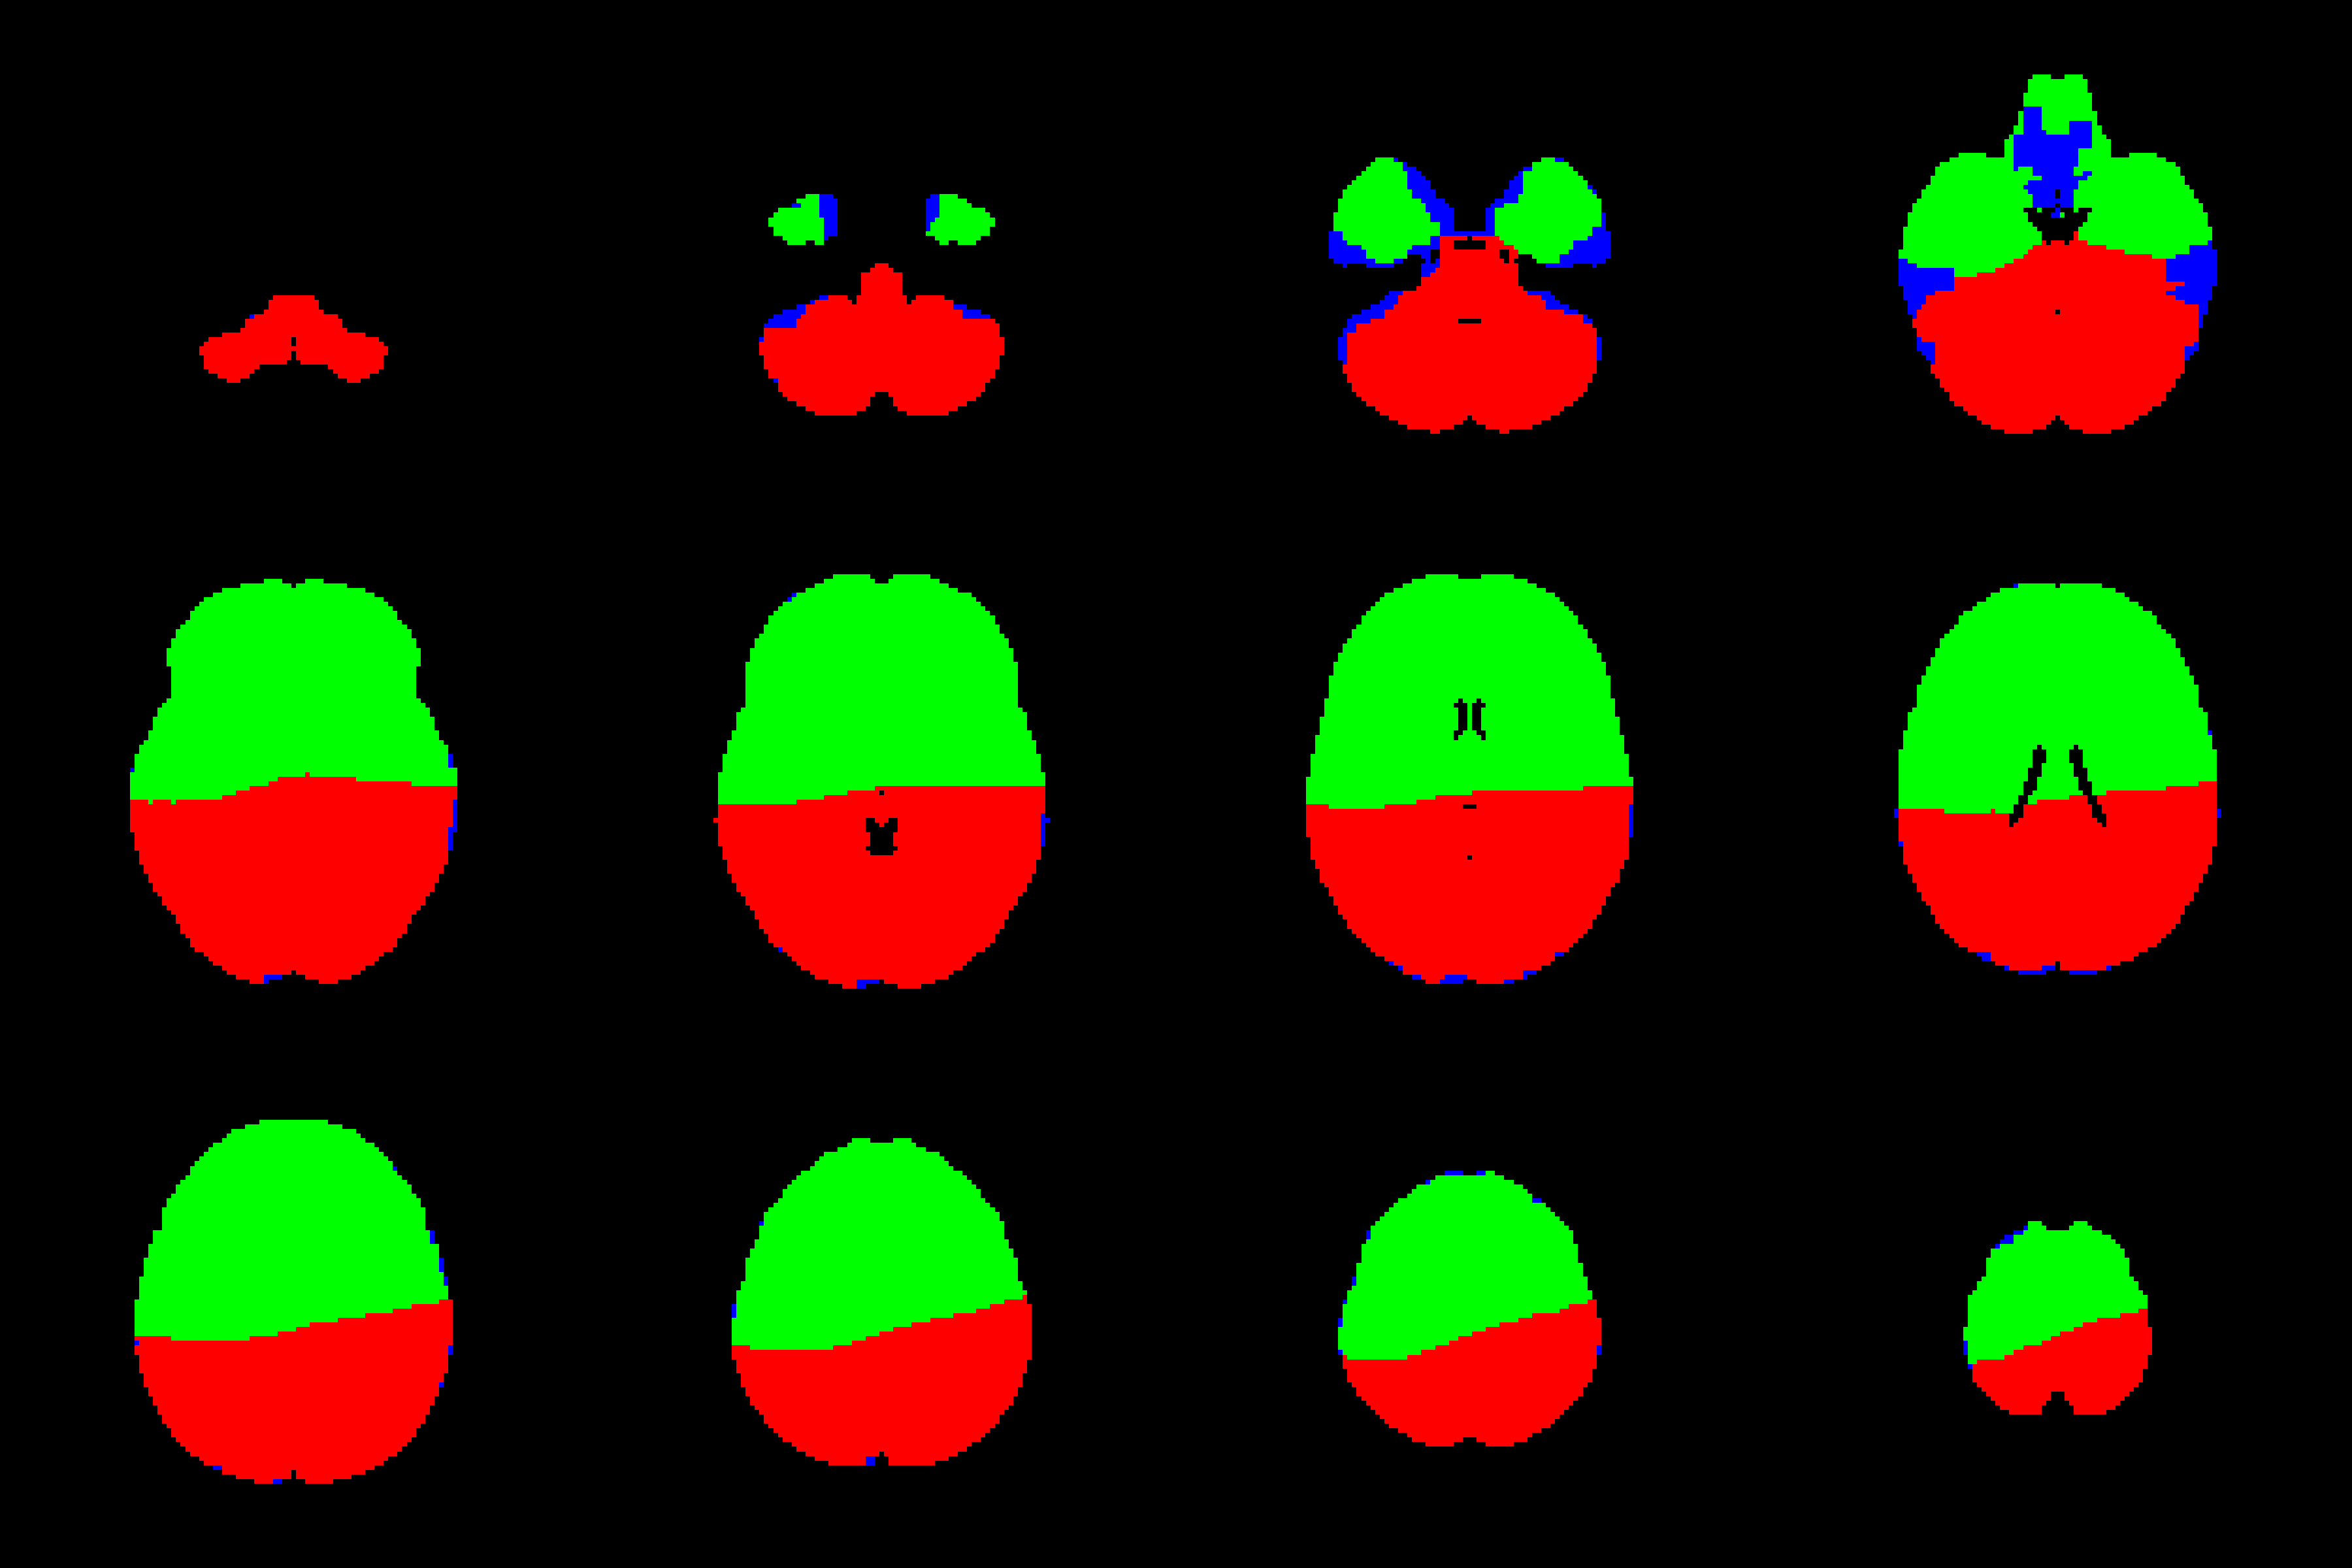
\includegraphics[scale = 0.5]{5_spectral_2_axial.png}

Axial

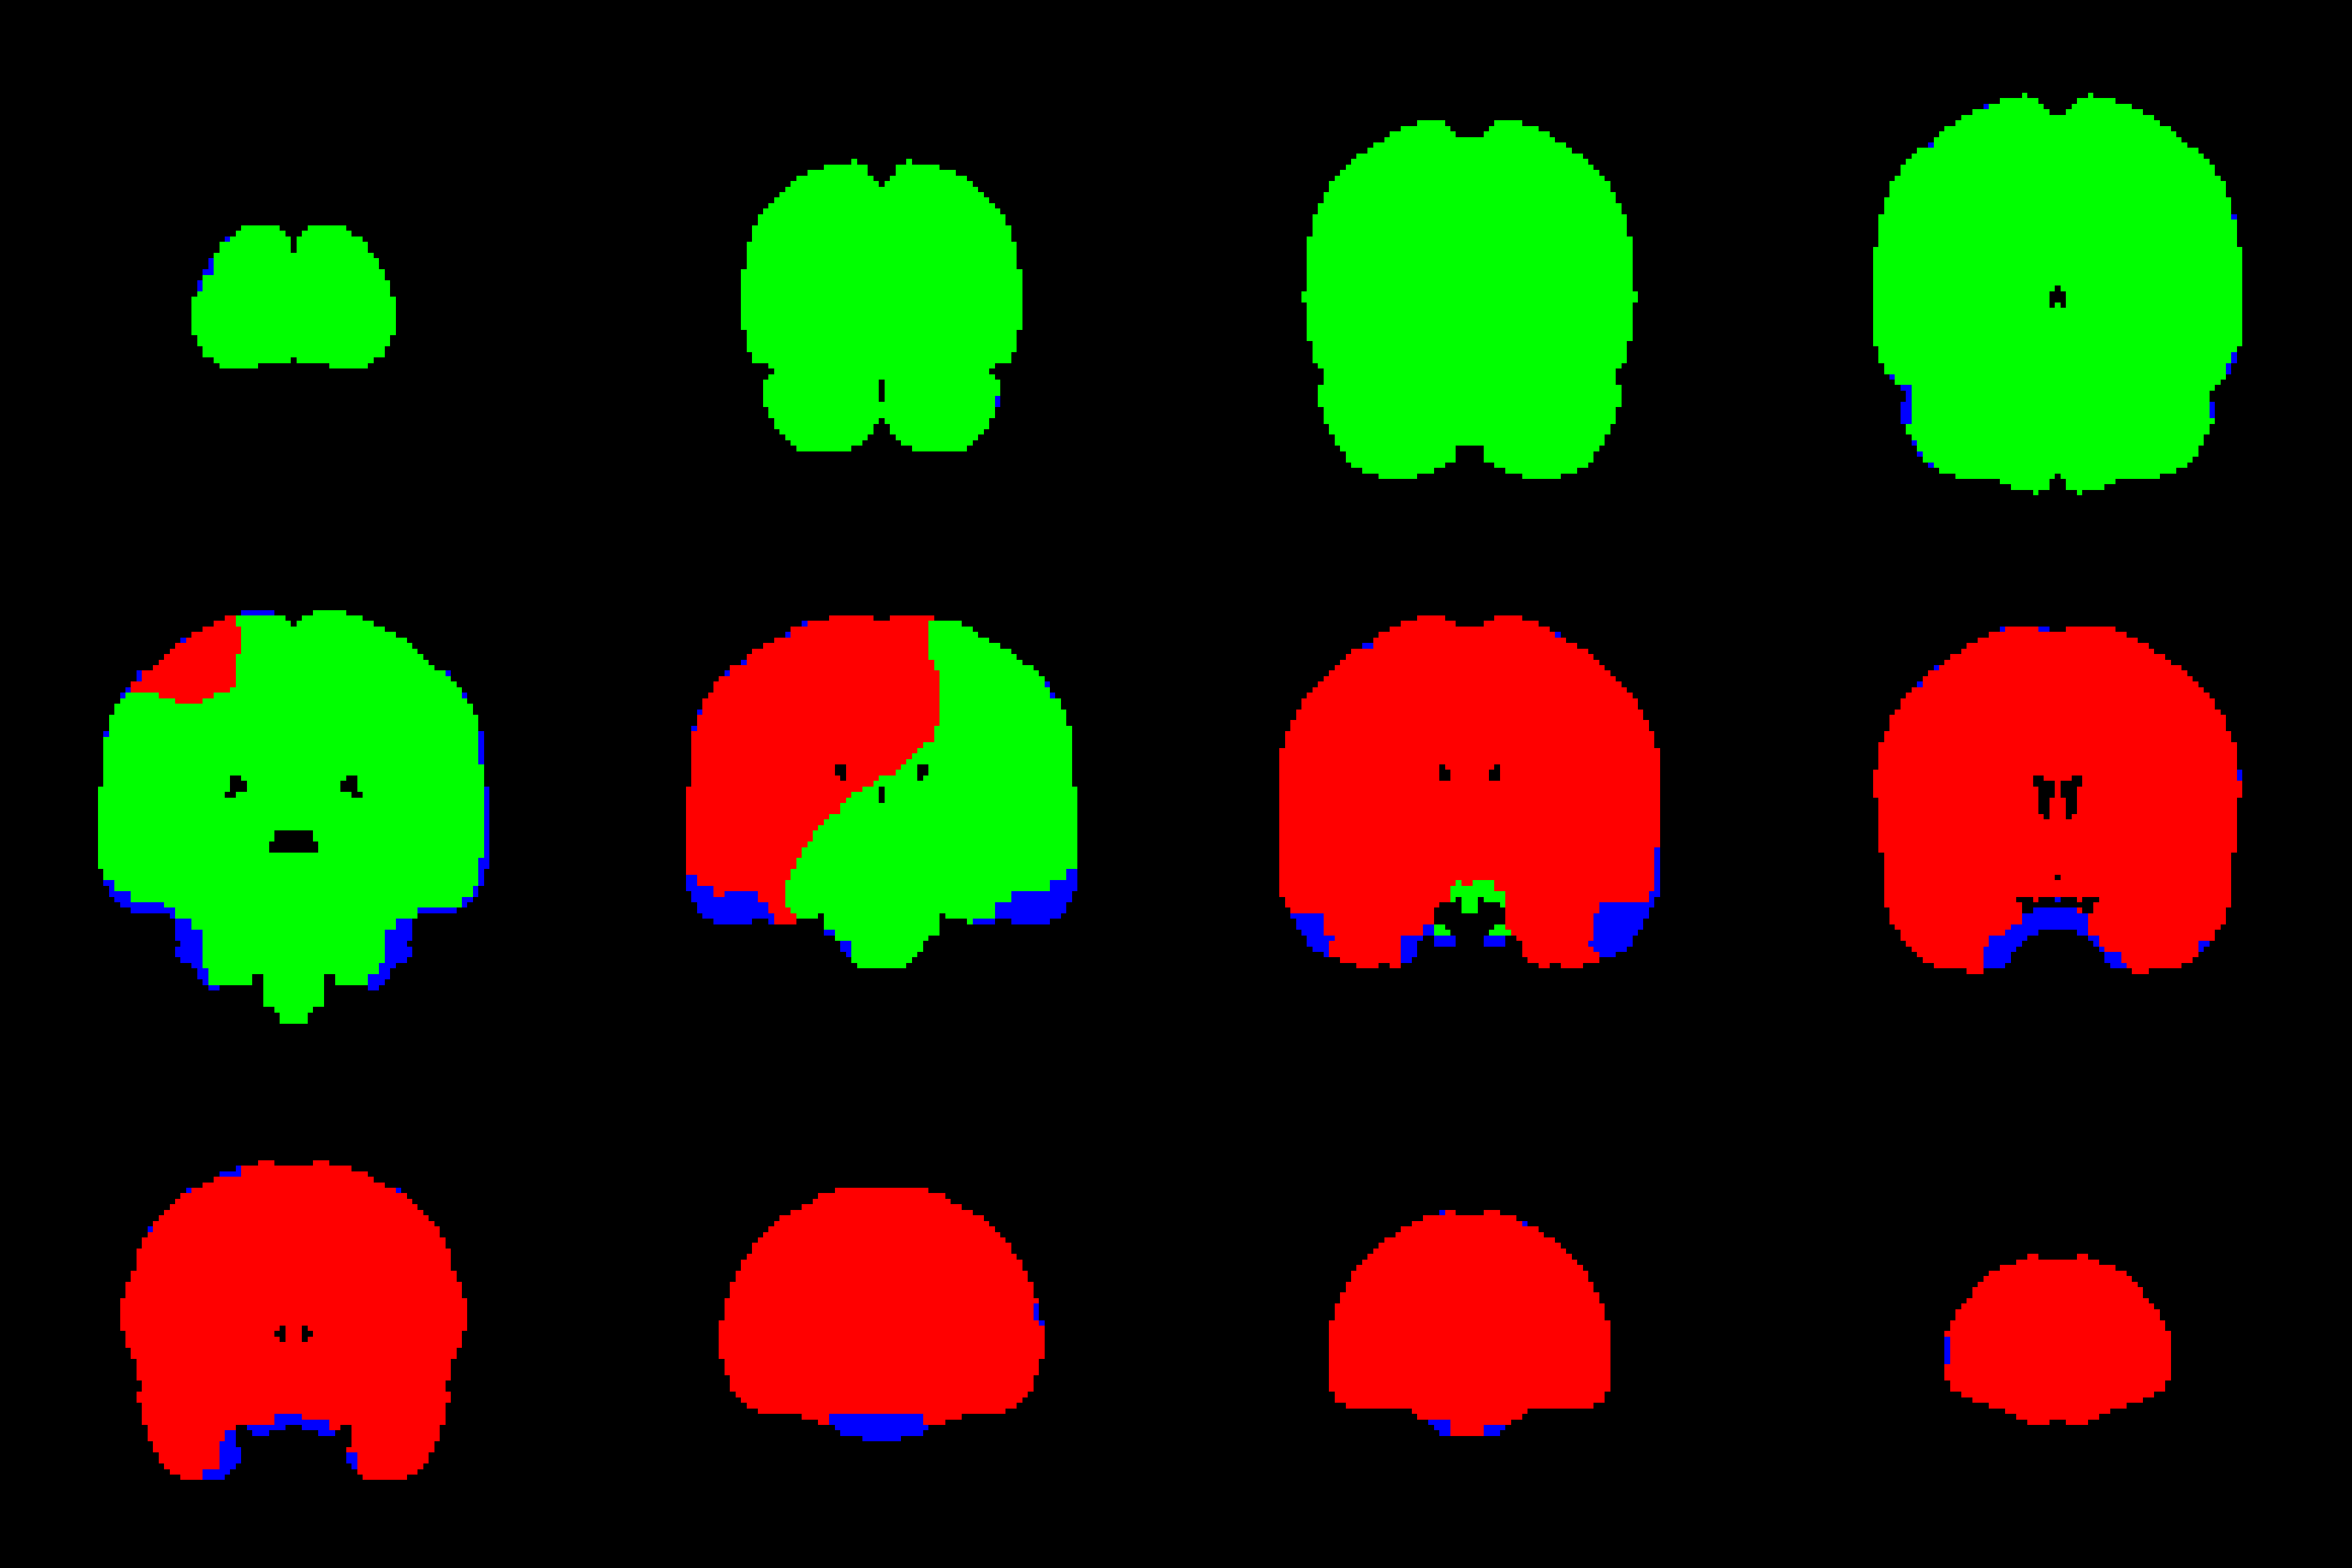
\includegraphics[scale = 0.5]{5_spectral_2_coronal.png}

Coronal

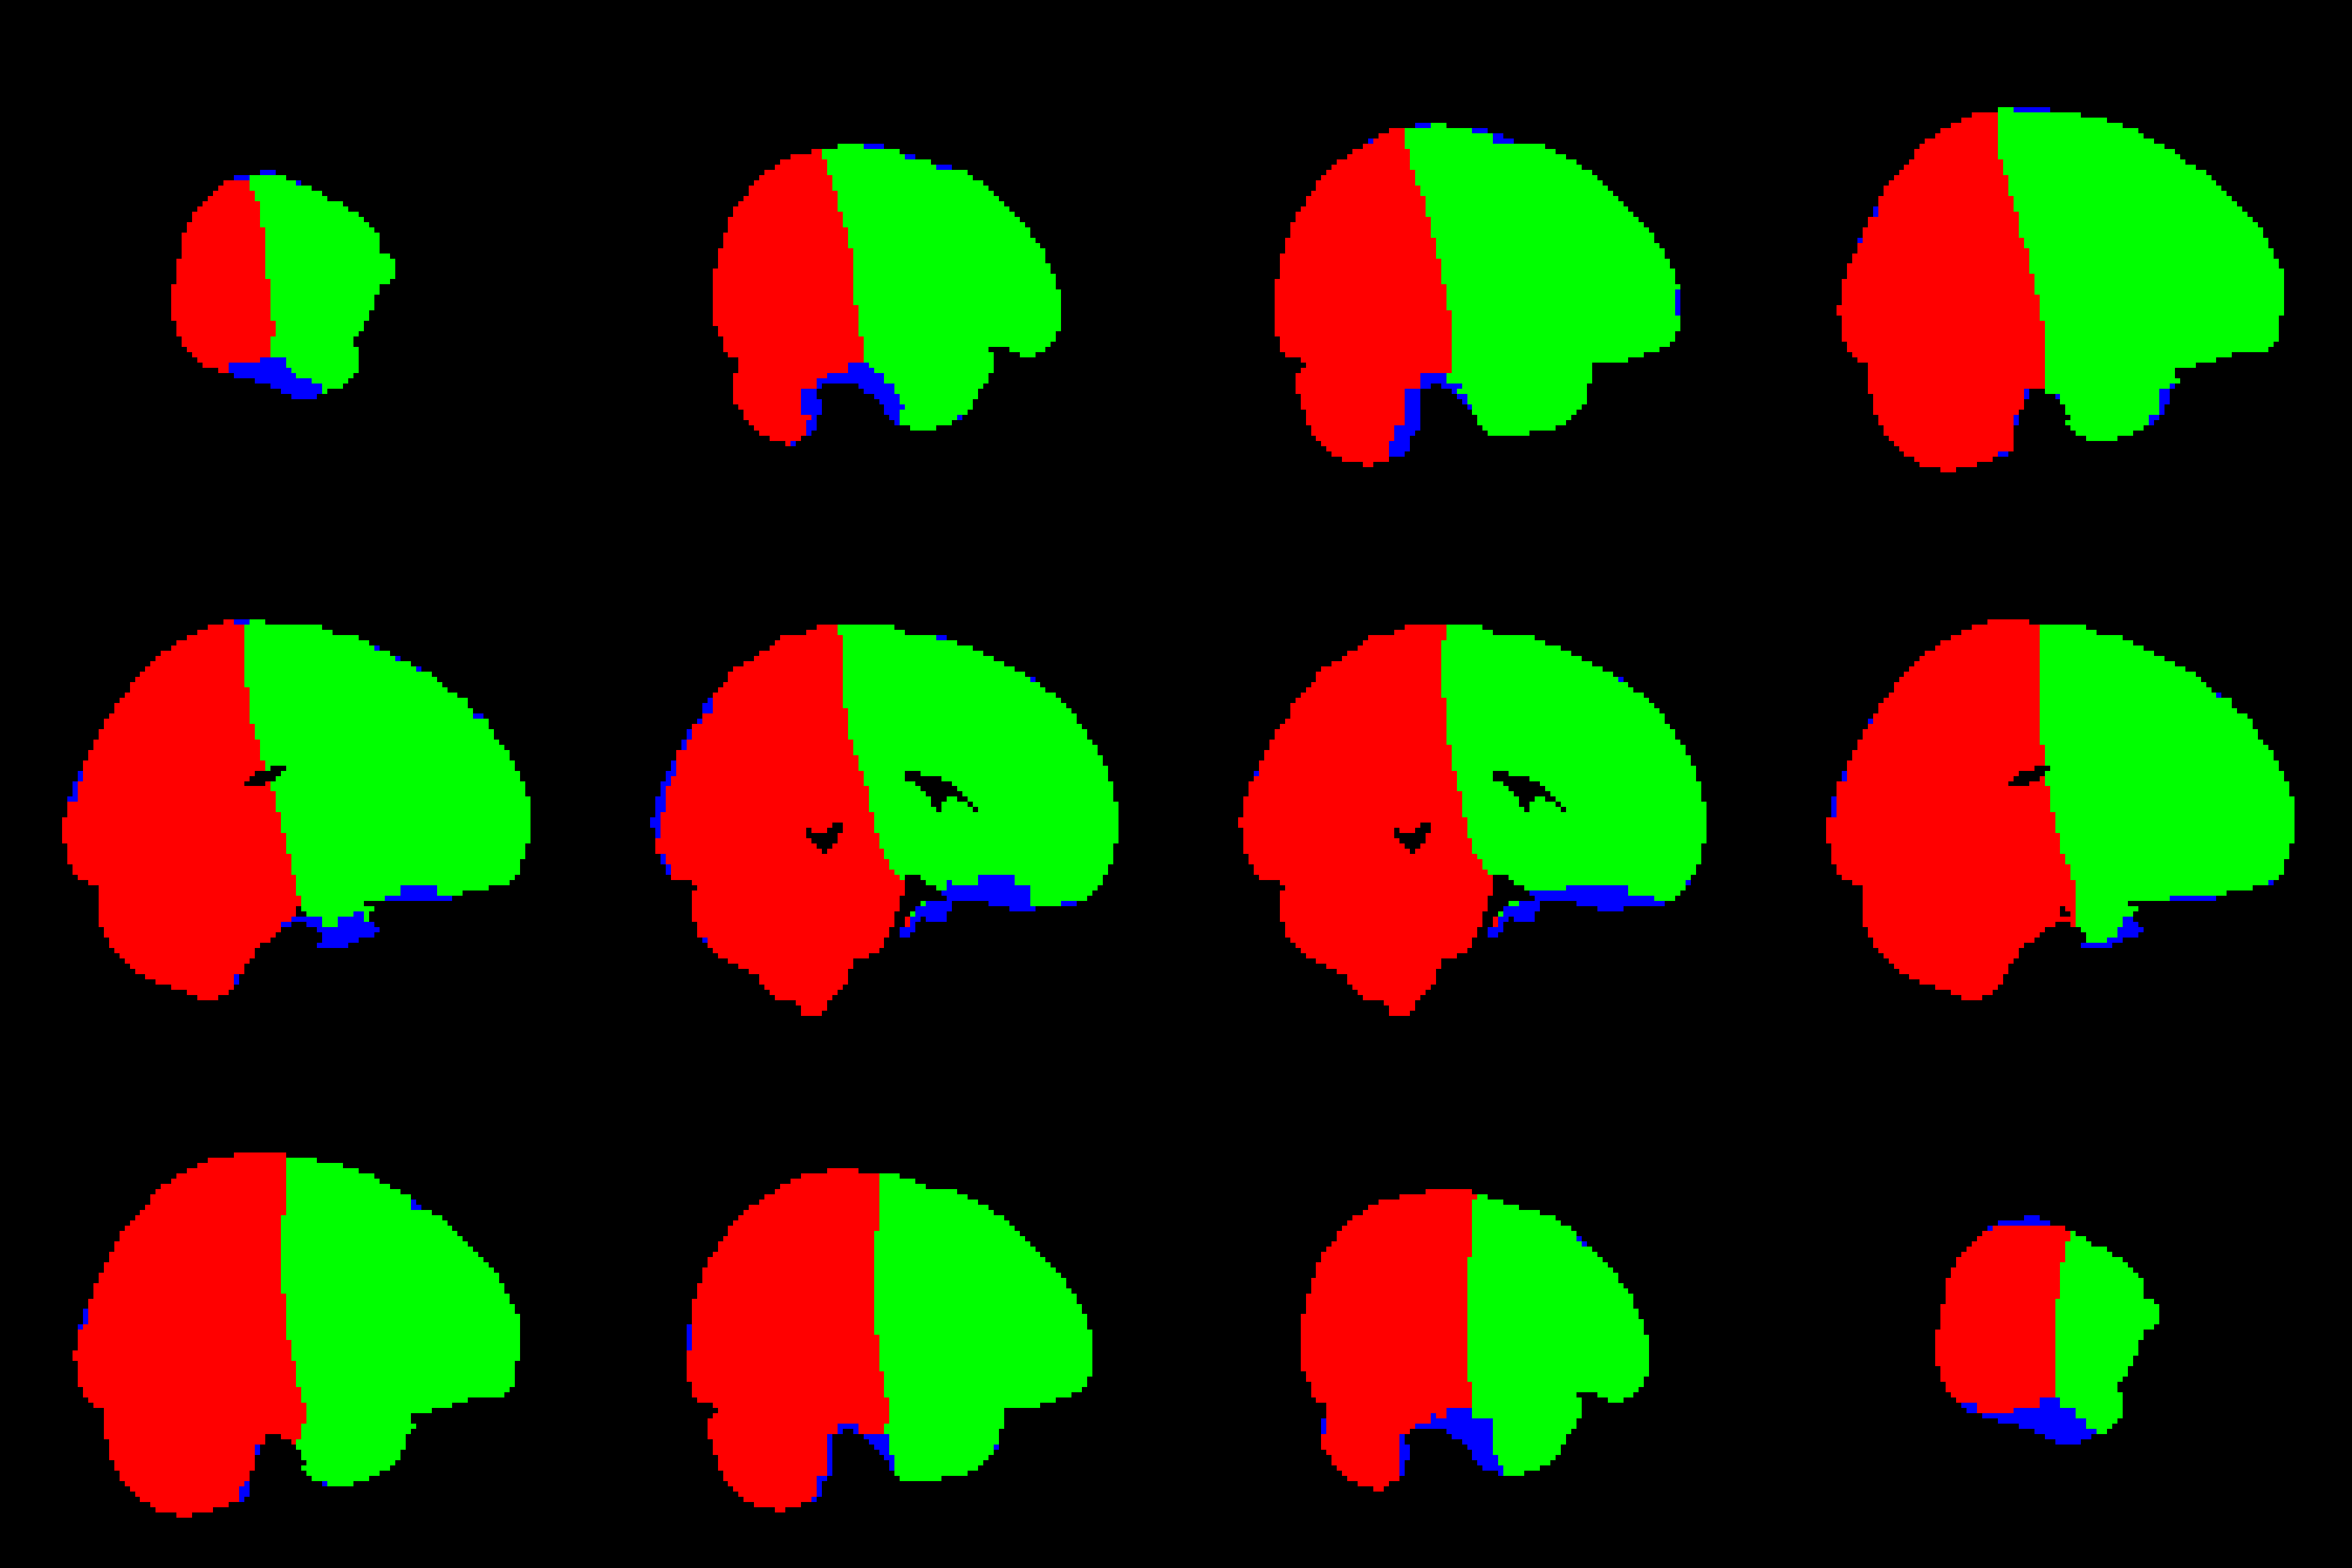
\includegraphics[scale = 0.5]{5_spectral_2_sagittal.png}

Sagittal
\end{center}

One can recursively apply this bipartitioning method to the component
subgraphs to obtain $k$-partitions, but there is a more elegant
approach involving additional eigenvectors that we shall discuss next.

\section{Spectral k-partitioning}


%#######################################################################


\chapter{Symmetric Nonnegative Matrix Factorization}
In the previous chapter, we showed that the problem of finding the
minimum ratio cut of a graph (with Laplacian matrix $L$, degree matrix
$D$, and adjacency matrix $A$) can be formulated as minimizing
\begin{equation} \label{ratio_cut}
\Tr(R^T L R)
\end{equation}
over the set, $\mathcal{R}$, of $n \times k$ matrices satisfying
\begin{enumerate}
\item
$R^T R = I$

\item
$R \geq 0$ (element-wise)

\item
$R R^T u_n = u_n$ where $u_n$ is a $n$-dimensional vector of all ones.
\end{enumerate}

If the sizes of the components in the optimal ratio cut partition
are perfectly balanced, which is equivalent to saying if the diagonal
of the optimal ratioed assignment matrix $R R^T$ has entries all
equal to $\frac{k}{n}$, then
\begin{align*}
\Tr(R^T D R) &= \sum_{i=1}^n [R R^T]_{ii} D_{ii} \\
             &= \sum_{i=1}^n \frac{k}{n} D_{ii} \\
             &= \frac{k}{n} \sum_{i,j} A_{ij}
\end{align*}
is a constant that does not depend on $R$. The same is true if each
vertex has the same degree $D_{ii} = d$, in which case
\begin{align*}
\Tr(R^T D R) &= \sum_{i=1}^n [R R^T]_{ii} D_{ii} \\
             &= d \sum_{i=1}^n [R R^T]_{ii} \\ 
             &= d k
\end{align*}
is also a constant that does not depend on $R$. In either case,
\[ \argmin{R \in \mathcal{R}} \Tr(R^T L R)
 = \argmax{R \in \mathcal{R}} \Tr(R^T A R) \]
This equality may also hold even if neither condition is true,
especially if they are approximately true.

Spectral $k$-partitioning drops the second and third constraints
of $\mathcal{R}$ to derive a closed-form minimizer of \ref{ratio_cut},
from which the original assignment matrix can be obtained by $k$-means.
This chapter deals with an alternative relaxation of $\mathcal{R}$ that
drops the first and third constraints.

\section{Nonnegative Matrix Factorization}

For an $n \times m$ matrix $A$, a nonnegative matrix factorization
(NMF) is a pair of matrices $W \in \R^{n \times k}$ and
$H \in \R^{m \times k}$ that minimizes $\| A - W H^T \|_F^2$
subject to elementwise nonnegativity: $H \geq 0$ and $W \geq 0$.
Here, $\|X\|_F = \sqrt{\sum_{ij} X_{ij}}$ refers to the Frobenius norm.

For $n \times n$ symmetric matrices $A$, a \textit{symmetric} NMF
(SymNMF) is a matrix $H \in \R^{n \times k}$ that minimizes
$\| A - H H^T \|_F^2$, and $k$ is an arbitrary positive integer
typically much smaller than $n$.

The following theorem from \cite{Ding:05} illustrates the connection
between SymNMF and graph partitioning.

\begin{theorem}
Let $A$ be a $n \times n$ symmetric matrix. Then
\[ \argmax{H^T H = I, H \geq 0} \Tr(H^T A H)
 = \argmin{H^T H = I, H \geq 0} \| A - H H^T \|_F^2 \]

Proof. \begin{align*}
   \argmax{H^T H = I, H \geq 0} \Tr(H^T A H)
&= \argmin{H^T H = I, H \geq 0} -2 \Tr(H^T A H) \\
&= \argmin{H^T H = I, H \geq 0} \Tr(A A^T) - 2 \Tr(H^T A H)
                                + \|H^T H\|_F^2 \\
&= \argmin{H^T H = I, H \geq 0} \|A - H H^T\|_F^2
\end{align*}
\end{theorem}

If $A$ is the adjacency matrix, then under the equal vertex degrees
condition described earlier
$ \argmax{H^T H = I, H \geq 0} \Tr(H^T A H)
= \argmin{H^T H = I, H \geq 0} \Tr(H^T L H)$.
Hence an alternative approach to the minimum ratio-cut problem
is to drop the $H^T H = I$ constraint and solve the SymNMF problem:

\begin{equation} \label{sym_nmf}
\begin{aligned}
\min_{H \in \R^{n \times k}} &\;& \|A - H H^T\|_F^2 \\
\text{s.t.}                  &\;& H \geq 0          \\
\end{aligned}
\end{equation}

This relaxation has two key differences from the spectral relaxation
\label{spectral_k-partition}.
\begin{itemize}
\item
There is no closed-form solution, and the optimal value is found
via an optimization algorithm, described in the next section.

\item
The optimal assignments are recovered directly from the largest
entry in each row. There is no need for $k$-means.
\end{itemize}

\section{An Alternating Nonnegative Least Squares Algorithm for SymNMF}

\cite{Kuang:15} re-formulates \ref{sym_nmf} as a non-symmetric NMF
with a penalty on the difference between the two matrix factors:
\[ \min_{W,H \geq 0}
   \|A - W H^T\|_F^2 + \alpha \|W - H\|_F^2
\]
where $W,H \in \R^{n \times k}$. The objective is equivalent to
\[ \norm{ \begin{bmatrix} W \\ \sqrt{\alpha} I_k \end{bmatrix} H^T
        - \begin{bmatrix} A \\ \sqrt{\alpha} W^T \end{bmatrix} }_F^2
\]

\chapter{Mixed Integer and Linear Programming}
We want to find a partitioning of graph $G(V,E)$ into $K$ components
so as to minimize the Adjacent-Score \ref{adjacent-score}
\[ \frac{1}{K} \sum_{V \in \mathcal{P}_K}
   \frac{1}{|E_{V,V}|} \sum_{(i,j) \in E_{V,V}} A_{i,j}
\]

Let $m = |E|$, the number of edges in the graph. Assign each edge an
index in $\{1, ..., m\}$ and 
let $a$ be an $m$-dimensional vector whose $j$th entry is the weight of
the $j$-indexed edge. Since distance correlation is between 0 and 1, so
are the entries of $a$.

For $k = 1, ..., K$, let $z_k \in \{0, 1\}^m$ be a 0-1 vector with
$j$th entry satisfying
\[ z_{jk} = \begin{cases}
  1 & \text{if both endpoints of edge } j \text{ are in } V_k
\end{cases} \]

If $z_1, ..., z_K \in \{0, 1\}^m$ describe a valid partitioning, then
they must satisfy $\sum_{k=1}^K z_{jk} \leq 1$ for all edges $j$.
However, the converse is not true, since this contraint still allows two
edges sharing an endpoint to be within different parcels.

To prevent that from happening, we introduce the assignment matrix
$X \in \{0, 1\}^{n \times m}$ with entries
\[ x_{i,k} = \begin{cases}
  1 & \text{if vertex } i \in V_k \\
  0 & \text{otherwise}
\end{cases} \]
and three constraints
\begin{align*}
1 + z_{jk} &\geq x_{hk} + x_{ik} \\
z_{jk} &\leq x_{hk} \\
z_{jk} &\leq x_{ik} \\
\end{align*}
for all $j = 1, ..., m$, $k = 1, ..., K$, where $(h,i)$ are the two
endpoints of edge $j$. If we constrain $X$ to be binary then the three
above constraints are equivalent to:
\[ z_{jk} = \begin{cases}
  1 & \text{if } x_{hk} = 1 \text{ and } x_{ik} = 1 \\
  0 & \text{otherwise} \\
\end{cases}\]
For the $X$, we only need to ensure every vertex is in a parcel and every
parcel has at least one vertex (or some other specified minimum):
\[ \sum_{k=1}^K x_{ik} = 1 \]
\[ \sum_{i=1}^n x_{ik} \geq 1 \]
where the equation holds for all $i$ and the inequality for all $k$.

Hence the following optimization problem finds a valid partition that
maximizes adjacent-score. Let $e_m$ denote a vector of $m$ ones.

\bgroup
\def\arraystretch{1.5}
\begin{tabular}{l l l}
maximize   & $\dfrac{a^T z_1}{e_m^T z_1} + \cdots +
              \dfrac{a^T z_K}{e_m^T z_K}$
\\ \\
subject to 
           & $\begin{cases}
                 1 + z_{jk} \geq x_{hk} + x_{ik} \\
                 z_{jk} \leq x_{hk}             \\
                 z_{jk} \leq x_{ik}             \\
             \end{cases}$
           & $j = 1, ..., m$, $k = 1, ..., K$, $(h,i) = j$ \\
           & $\sum_{j=1}^m z_{jk} \geq 1$ & $k = 1, ..., K$ \\
           & $\sum_{k=1}^K x_{ik} = 1$ & $i = 1, ..., n$ \\
           & $\sum_{i=1}^n x_{ik} \geq 1$ & $k = 1, ..., K$ \\
           & $X \in \{0, 1\}^{n \times K}$
\end{tabular}
\egroup

Following the result in \cite{Li:94} we derive an equivalent Mixed Binary
Linear Program to the above.
Substitute $y_k = \dfrac{1}{e_m^T z_k}$ for each $k$, which amounts to
introducing a new variable $y \in \R^m$ and non-linear constraints
\[ e_m^T z_k y_k = 1 \]
The key theorem in \cite{Li:94} uses the fact that $z_k$ is binary to
linearize this contraint by introducing another variable $w_{jk}$ and
using linear constraints to enforce the nonlinear $w_{jk} = z_{jk} y_k$.
There are four linear constraints for each $w_{jk}$:

\begin{enumerate}
\item
$y_j - w_{jk} \leq 1 - z_{jk} $
\item
$w_{jk} \leq y_j$
\item
$w_{jk} \leq z_{jk}$
\item
$w_{jk} \geq 0$ 
\end{enumerate}

If $z_{jk} = 1$, then 1 and 2 will ensure that $w_{jk} = y_k$.
If $z_{jk} = 0$, then 3 and 4 will ensure that $w_{jk} = 0$.
It is important to note that this construction wouldn't work if
$y_k > 1$. In our case, this occurs if and only if $z_{jk} = 0$ for all
$j$, which has already been excluded by $\sum_{j=1}^m z_{jk} \geq 1$.

Now we are ready to present the mixed integer version

\bgroup
\def\arraystretch{1.5}
\begin{tabular}{l l l}
maximize   & $a^T w_1 + \cdots + a^T w_K$
\\ \\
subject to 
           & $\begin{cases}
                 1 + z_{jk} \geq x_{hk} + x_{ik} \\
                 z_{jk} \leq x_{hk}             \\
                 z_{jk} \leq x_{ik}             \\
             \end{cases}$
           & $j = 1, ..., m$, $k = 1, ..., K$, $(h,i) = j$ \\
           & $\sum_{j=1}^m z_{jk} \geq 1$ & $k = 1, ..., K$ \\
           & $\sum_{k=1}^K x_{ik} = 1$ & $i = 1, ..., n$ \\
           & $\sum_{i=1}^n x_{ik} \geq 1$ & $k = 1, ..., K$ \\
           & $X \in \{0, 1\}^{n \times K}$ \\
           & $\sum_{j=1}^m w_{jk} = 1$ & $k = 1, ..., K$ \\
           & $\begin{cases}
                y_j - w_{jk} \leq 1 - z_{jk} \\
                w_{jk} \leq y_j \\
                w_{jk} \leq z_{jk} \\
                w_{jk} \geq 0 \\
             \end{cases}$
           & $j = 1, ..., m$, $k = 1, ..., K$
\end{tabular}
\egroup

which can be solved globally by branch-and-bound methods.
Unfortunately the size of our graph is too large for a generic MIP
solver, and the largest graphs we partitioned using this method had
around 400 vertices and 3000 edges, partitioned into 10 components.
This is true even when the binary $\{0, 1\}$ constraint was relaxed
to an interval $[0, 1]$ to create an LP.

A faster approximation with fewer variables to this MIP involves
dropping the assignment matrix $X$.

\section{Other Objectives}


\chapter{Results}
{\color{red}Some lead into here.}

\section{Summary of Methods}

\begin{table}
\caption{Summary of Partitioning Methods}
\label{8_methods}
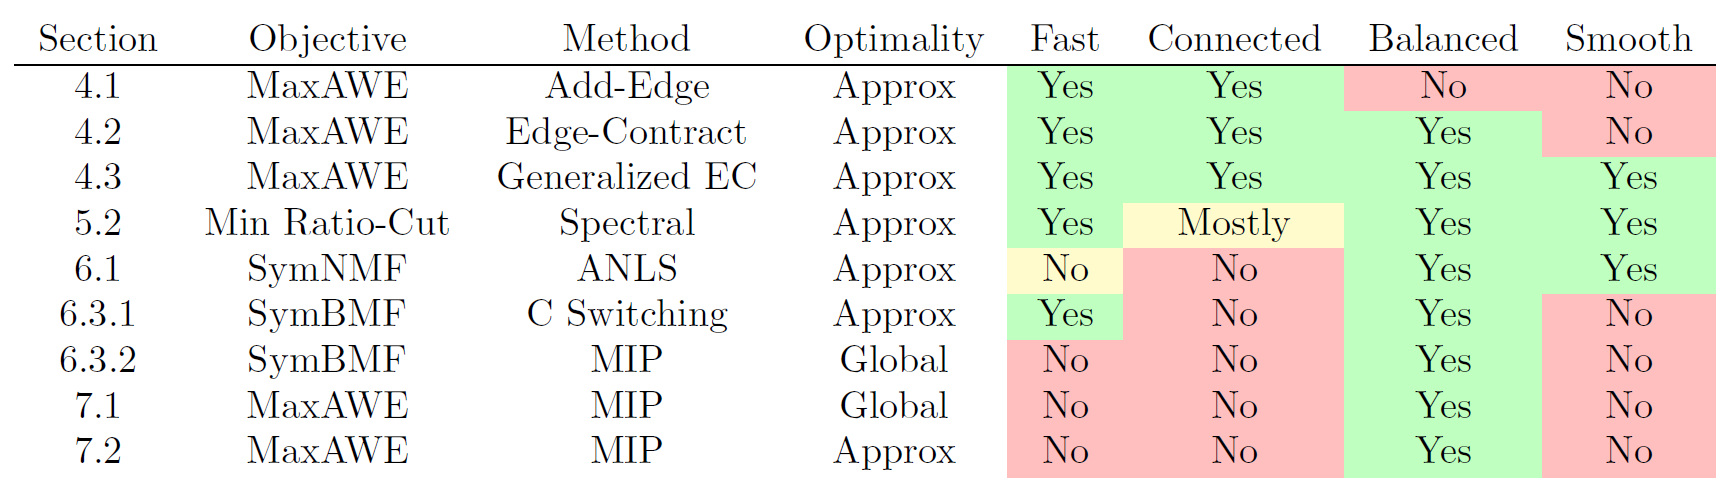
\includegraphics[scale = 0.5]{figs/8_methods.png}
%\begin{tabular}{cccccccc}
%Section & Objective & Method & Optimality & Fast & Connected & Balanced & Smooth \\
\hline
4.1 & MaxAWE & Add-Edge & Approx & \cellcolor{green!25}Yes & \cellcolor{green!25}Yes & \cellcolor{red!25}No & \cellcolor{red!25}No \\
4.2 & MaxAWE & Edge-Contract & Approx & \cellcolor{green!25}Yes & \cellcolor{green!25}Yes & \cellcolor{green!25}Yes & \cellcolor{red!25}No \\
4.3 & MaxAWE & Generalized EC & Approx & \cellcolor{green!25}Yes & \cellcolor{green!25}Yes & \cellcolor{green!25}Yes & \cellcolor{green!25}Yes \\
5.2 & Min Ratio-Cut & Spectral & Approx & \cellcolor{green!25}Yes & \cellcolor{yellow!25}Mostly & \cellcolor{green!25}Yes & \cellcolor{green!25}Yes \\
6.1 & SymNMF & ANLS & Approx & \cellcolor{yellow!25}No & \cellcolor{red!25}No & \cellcolor{green!25}Yes & \cellcolor{green!25}Yes \\
6.3.1 & SymBMF & C Switching & Approx & \cellcolor{green!25}Yes & \cellcolor{red!25}No & \cellcolor{green!25}Yes & \cellcolor{red!25}No \\
6.3.2 & SymBMF & MIP & Global & \cellcolor{red!25}No & \cellcolor{red!25}No & \cellcolor{green!25}Yes & \cellcolor{red!25}No \\
7.1 & MaxAWE & MIP & Global & \cellcolor{red!25}No & \cellcolor{red!25}No & \cellcolor{green!25}Yes & \cellcolor{red!25}No \\
7.2 & MaxAWE & MIP & Approx & \cellcolor{red!25}No & \cellcolor{red!25}No & \cellcolor{green!25}Yes & \cellcolor{red!25}No \\

%\end{tabular}
\end{table}

Table (\ref{8_methods}) summarizes the objectives, advantages, and
drawbacks of each partitioning method we've presented in the previous
chapters. Clearly, the requirement of parcels to be connected components
is the biggest roadblock to developing a good method.

There is a post-processing method that can take a parcellation with
disconnected components and modify it to be connected. The method is to
treat each separate component of a parcel as new parcels, create a
Contractible Graph with these new parcels as components, and apply the
(Generalized) Edge Contract algorithm. This was carried out as a
post-processing step in the spectral and SymBMF parcellations, detailed
in the next section.

The second limiting factor is computational time. The Alternating
Nonnegative Least Squares algorithm can be made to work on graphs as
large as the brain, but this would require some specialized data
structures for the computation of $X$ and $Y$ to avoid re-computing
unchanged columns. Unfortunately we did not have enough time to
implement this.

The problem of computational time is most evident in the integer (and
linear) programming methods. The fact that our brain data was too large
for even the lightest linear program shows that this generic
optimization approach is typically not feasible. However, these
proposed methods may be of use to problems with smaller data sets.

One possible approach to dealing with computational time that we have
not had the time to explore is to apply the MIP methods to small
subgraphs of the brain. For instance, one could take the AAL
parcellation and obtain a finer parcellation by using a MIP method on
each of the AAL parcels.

The only method that satisfies the requirements of computational speed,
parcel connectedness, size balance, and smoothness without any
post-processing steps is the Generalized Edge-Contraction family of
algorithms. In the next section we will show that it is also the
parcellation method that produces the best Adjacent-Scores.

All of the methods above can be applied to the similar problem of
\textit{clustering}. In fact, similarity-based clustering is just a
special case of graph partitioning where the graph is fully connected
(i.e., every vertex has an edge to every other vertex), so connectedness
of partitions is no longer a relevant factor. Then, if we define the
Adjacent-Score in terms of similarity equal to negative Euclidean
distance squared
\[ \frac{1}{K}\sum_{k=1}^K \frac{1}{{|V_k| \choose 2}}
   \sum_{x,y \in V_k} - \|x - y\|^2, \]
the objective of maximizing Adjacent-Score becomes equivalent to 
minimizing a weighted within-cluster sum of squares objective
\[ \sum_{k=1}^K \frac{1}{{|V_k| \choose 2}}
   \sum_{x \in V_k} \|x - \mu_k\|^2 \]
where $\mu_k$ is the mean of all $x$ in $V_k$.

{\color{red}It'll be nice to cite the equations in Chapter 3 for
the criterion values}

\section{Parcellations of ABIDE fMRI Scans}

\begin{table}
\caption{Criteria Scores of Various Parcellation Methods, %
Averaged Across Normal Brains}
\label{normal}
\begin{tabular}{l | r r r r r r}
& \rot{Adjacent}
& \rot{Boundary}
& \rot{RatioCut}
& \rot{CompParc}
& \rot{Balance}
& \rot{Jaggedness}
\\ \hline
GenEC (3,1)         & 0.766 & 0.799 & 47.118 & 1     & 0.251 & 23.930 \\
GenEC (6,1)         & 0.774 & 0.796 & 51.342 & 1     & 0.280 & 28.801 \\
GenEC (6,4)         & 0.773 & 0.800 & 51.285 & 1     & 0.335 & 29.199 \\
Spectral            & 0.747 & 0.810 & 43.242 & 1.027 & 0.728 & 16.347 \\
Spectral GenEC(6,4) & 0.747 & 0.810 & 43.162 & 1     & 0.713 & 16.305 \\
SymBMF      & 0.845 & 0.962 & 293.662 & 470.994 & 0.838 & 305.302 \\
SymBMF GenEC(6,4)   & 0.773 & 0.798 & 53.256 & 1     & 0.290 & 30.086 \\

\end{tabular}
\end{table}

\begin{table}
\caption{Criteria Scores of Various Parcellation Methods, %
Averaged Across Autism Spectrum Brains}
\label{autism}
\begin{tabular}{l | r r r r r r}
& \rot{Adjacent} & \rot{Boundary} & \rot{RatioCut} & \rot{CompParc} & \rot{Balance} & \rot{Jaggedness} \\
\hline
GenEC (3,1) & 0.762 & 0.821 & 46.615 & 1 & 0.210 & 25.008 \\
GenEC (6,1) & 0.769 & 0.827 & 51.613 & 1 & 0.249 & 31.178 \\
GenEC (6,4) & 0.771 & 0.821 & 51.705 & 1 & 0.309 & 31.821 \\
Spectral    & 0.739 & 0.827 & 42.464 & 1.024 & 0.697 & 16.36 \\
Spectral GenEC(6,4) & 0.739 & 0.827 & 42.427 & 1 & 0.677 & 16.333 \\
SymBMF & 0.844 & 0.969 & 289.129 & 473.102 & 0.827 & 306.992 \\
SymBMF GenEC(6,4) & 0.769 & 0.821 & 52.742 & 1 & 0.261 & 31.927 \\

\end{tabular}
\end{table}

Tables (\ref{normal}) and (\ref{autism}) respectively show the results
of various parcellation methods carried out on resting state fMRI scans
of 6 control and 6 autism patients. The number of parcels in each
method is set to 116, the same as AAL. Each brain was preprocessed to
remove vertices with edge weights of 0 to all adjacent vertices. For
each method and criterion, the values are averaged over the six 
subjects in each cohort. In our methods, SymBMF was carried out using
component switching on the incomplete adjacency matrix (only
approximation of non-zero entries in the $A$ matrix was considered).
GenEC ($\alpha$, $\beta$) denotes a Generalized Edge-Contract
algorithm using standard priority function (\ref{priority_func}) with
parameters $\alpha$ and $\beta$. When this is written after a different
method such as Spectral, it means we post-processed the Spectral
parcellation using GenEC to obtain connected parcels.

Despite producing a parcellation with the highest Adjacent-Score, the
Component Switching SymBMF method is the least suitable for parcellation
since its parcels are extremely fragmented, with an average 473
components per parcel. The reason for this is that the adjacency matrix
was treated as incomplete, so there was no penalty for a vertex
belonging to a parcel with many vertices it is disconnected from.
The high Adjacent-Score of SymBMF parcellations suggests a trade-off
between maximizing weights of within edges and creating connected and
smooth parcels.

The other parcellations aside from pure SymBMF has CompParc, Balance,
and Jaggedness scores that were at least as good as the AAL ones.
The Spectral parcellations were the smoothest, as expected, but this
came at the cost of lower Adjacent-Score and higher Boundary-Score
relative to the GenEC parcellations.
In both groups, the Generalized Edge-Contract with parameters
$\alpha = 6$ and $\beta = 4$ performed best. These parcellations had
the highest Adjacent-Scores and while maintaining Balance and
Jaggedness Scores close to those of the AAL. There is no significant
difference in the parcellation results of autism and control brains.

\section{Reproducibility of Parcellations and Cross-Validation}

\begin{figure}
\caption{Adjusted Rand Index Between Different 116-Parcel %
Parcellations of the same fMRI Scan, Averaged over All Subjects}
\label{ari_same}
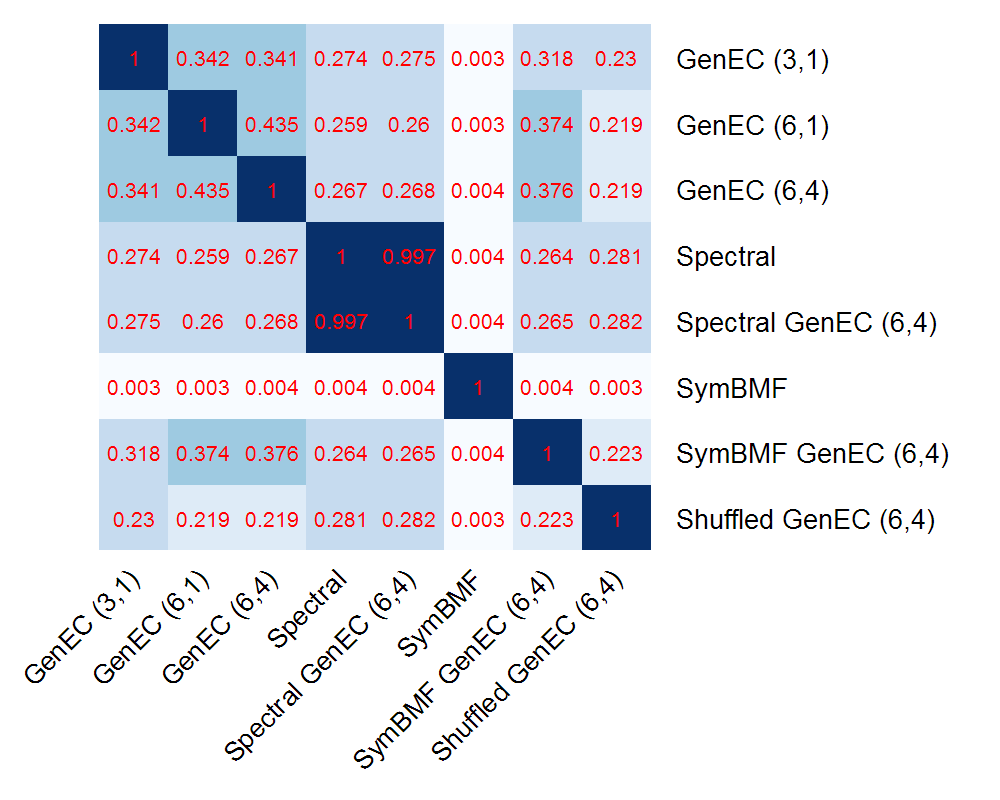
\includegraphics[scale = 1]{figs/8_ari_same.png}
\end{figure}

\begin{figure}
\caption{Adjusted Rand Index Between 116-Parcel GenEC(6,4)
Parcellations on Different fMRI Scans}
\label{ari_diff}
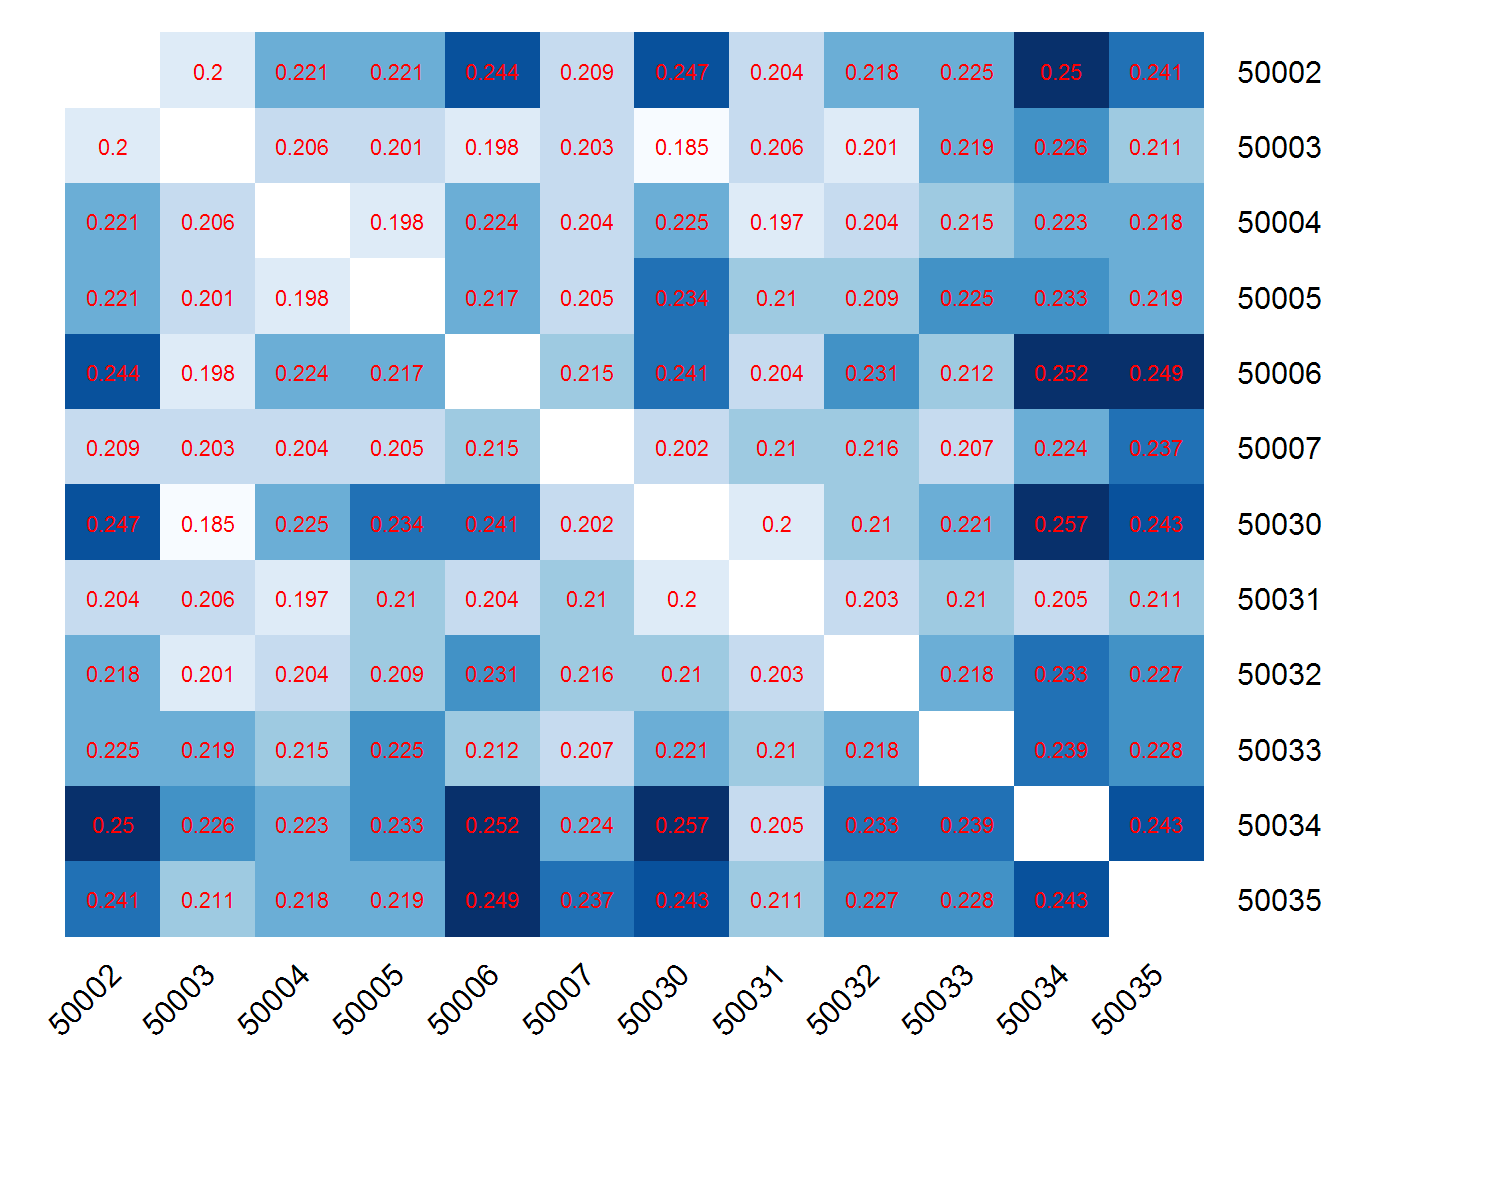
\includegraphics[scale = 0.95]{figs/8_ari_diff.png}
\end{figure}

We measured the similarity of 116-parcel parcellations from different
methods on the same brain, across brains in the control and autistic
cohorts. We used the Adjusted Rand Index \ref{ari} {\color{red}Citation doesn't
work} as our measure of
similarity, where 1 means identical parcel assignments and 0 means no
different from random parcel assignments. The result is shown in Figure
(\ref{ari_same}). The last row and column refer to ARI values with
respect to a random parcellation, generated by applying GenEC (6,4) to
the same brain graph with edge weights shuffled. The reason for this is
to account for the portion of ARI scores that derive solely from the
connectedness and smoothness property of parcellations.

As expected, the first three GenEC parcellations are similar to one
another, more than they are to the shuffled parcellation or to the
Spectral parcellations. The SymBMF GenEC (6,4) parcellation can also be
grouped with the first three. The unconnected SymBMF parcellation is
similar to no other since it is too fragmented.

Next, we restricted ourselves to the GenEC (6,4) method and measured
how similar the parcellations this method produced on different brains
are. The results are shown in Figure (\ref{ari_diff}). From Figure
(\ref{ari_same}) we know that the ARI between a GenEC (6,4) parcellation
on a shuffled brain graph and an actual one is around 0.219.
Surprisingly, for nearly all pairs of brains, the ARI value between
their GenEC (6,4) parcellations is no greater than this. We also see
that the mean ARI between autistic and control brains is not
significantly different from the mean ARI between brains of the same
cohort at the 116-parcel level. This suggests too much variation in the
spatial distribution of distance correlations across the edges of
different brain graphs for there to be a common parcellation fitting
all brains.

\begin{figure}
\caption{Difference of Adjacent-Score, Cross-Validation of 116-Parcel
GenEC (6,4) Parcellation on 12 Autism and Control Brains}
\label{cv_ec}
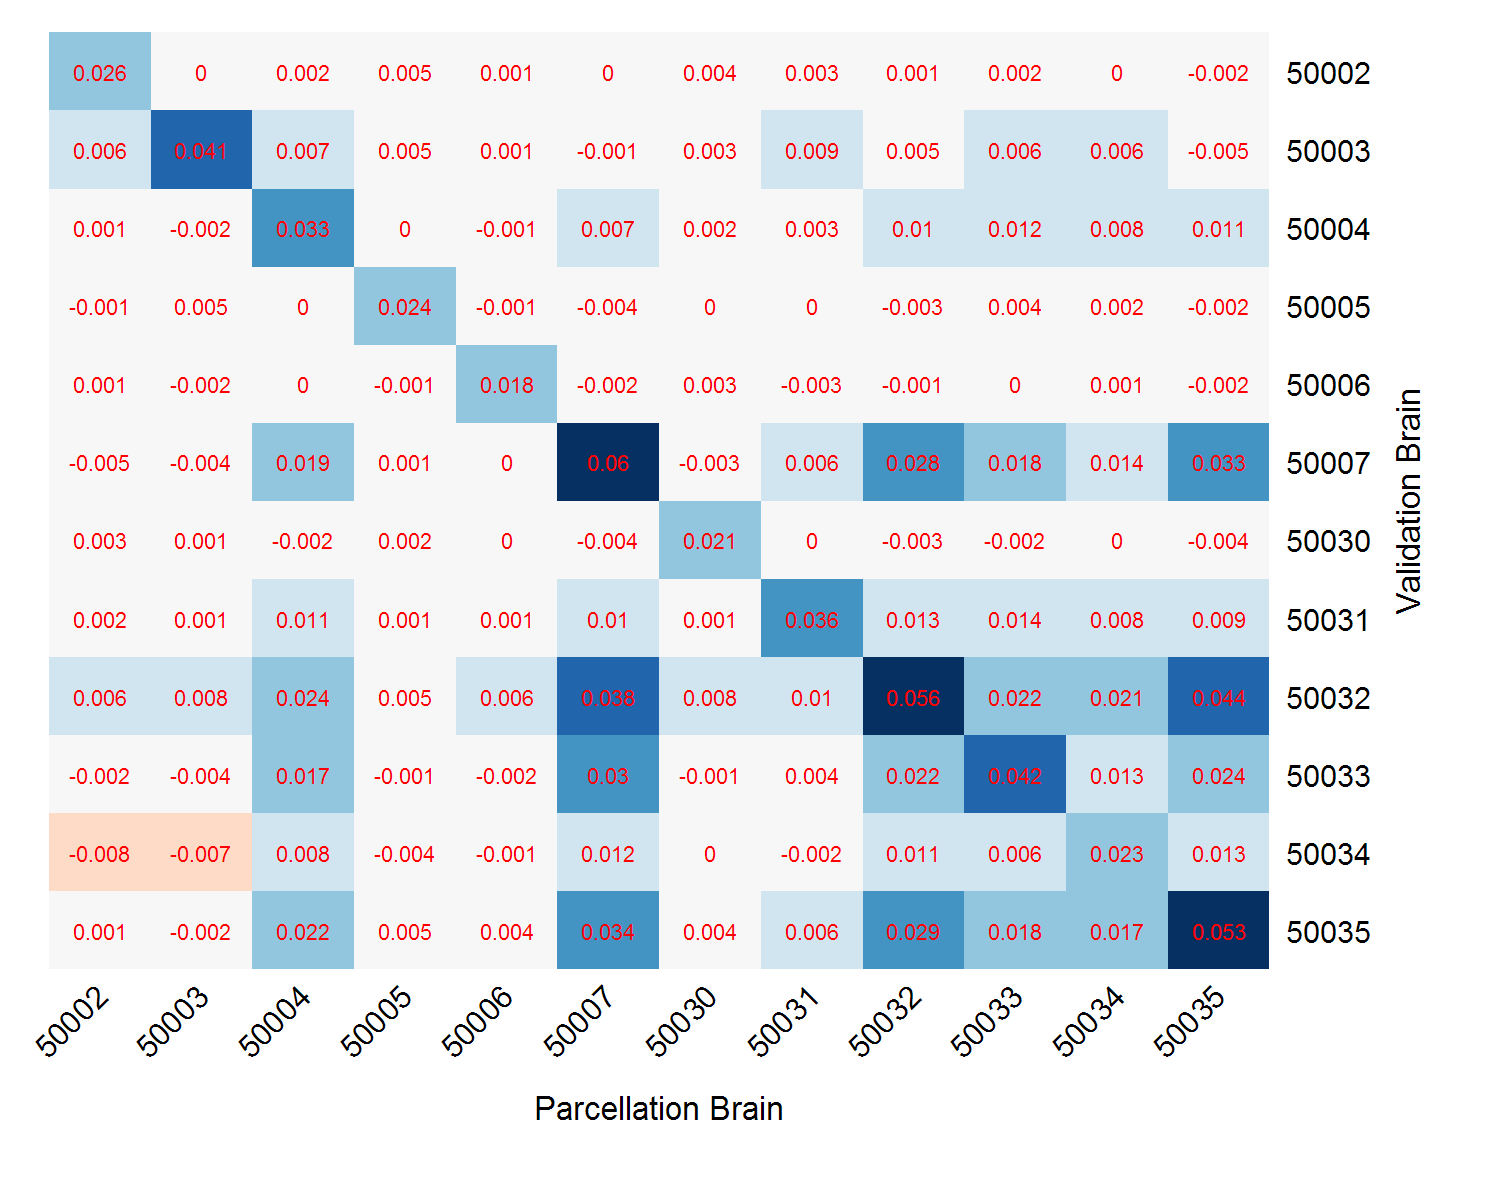
\includegraphics[scale = 1]{figs/8_cv_ec.png}
\end{figure}

To verify this, we conducted a cross-validation procedure where
for each pair of brains, we let one be the parcellation brain and one
be the validation brain. On the parcellation brain we performed two
parcellations: GenEC (6,4) and Shuffled GenEC (6,4) for the control.
On the validation brain we computed the Adjacent-Scores of both
parcellations. We stored the difference GenEC minus Shuffled in a
12 by 12 matrix, displayed in Figure (\ref{cv_ec}). The diagonal values
are in-sample Adjacent-Scores where the parcellation brain and the
validation brain are the same.

Assuming normality, a one sample t-test of the mean non-diagonal
cross-validation value shows that it is significantly greater than 0
($p \leq 2.2 \times 10^{-16}$). This indicates some degree of similarity
between different brains in the statistical dependencies of adjacent
voxels. Furthermore, Welch's two sample t-test of unequal variances
tells us the mean off-diagonal CV value in the autism cohort and the
control cohort are unequal ($p = 0.0138$). The control group has a
higher realized mean. These observations can serve as a basis for
further study.

Finally, we investigate whether the GenEC (6,4) parcellations could be
overfitting. The GenEC methods produced parcellations that scored well
in-sample (diagonal mean 0.048) but not as well out-of-sample
(off-diagonal mean 0.010), so it is possible that the parcellations
they produce are too flexible. To see if this could be the case, we
perform the same cross-validation procedure except now using the
spectral method. The reason for this is that partitions obtained via the
spectral method have lower Jaggedness values and smoother surfaces,
and hence are less likely to overfit the graph.

\begin{figure}
\caption{Difference of Adjacent-Score, Cross-Validation of
116-Parcel Spectral Parcellation on 12 Autism and Control Brains}
\label{cv_sp}
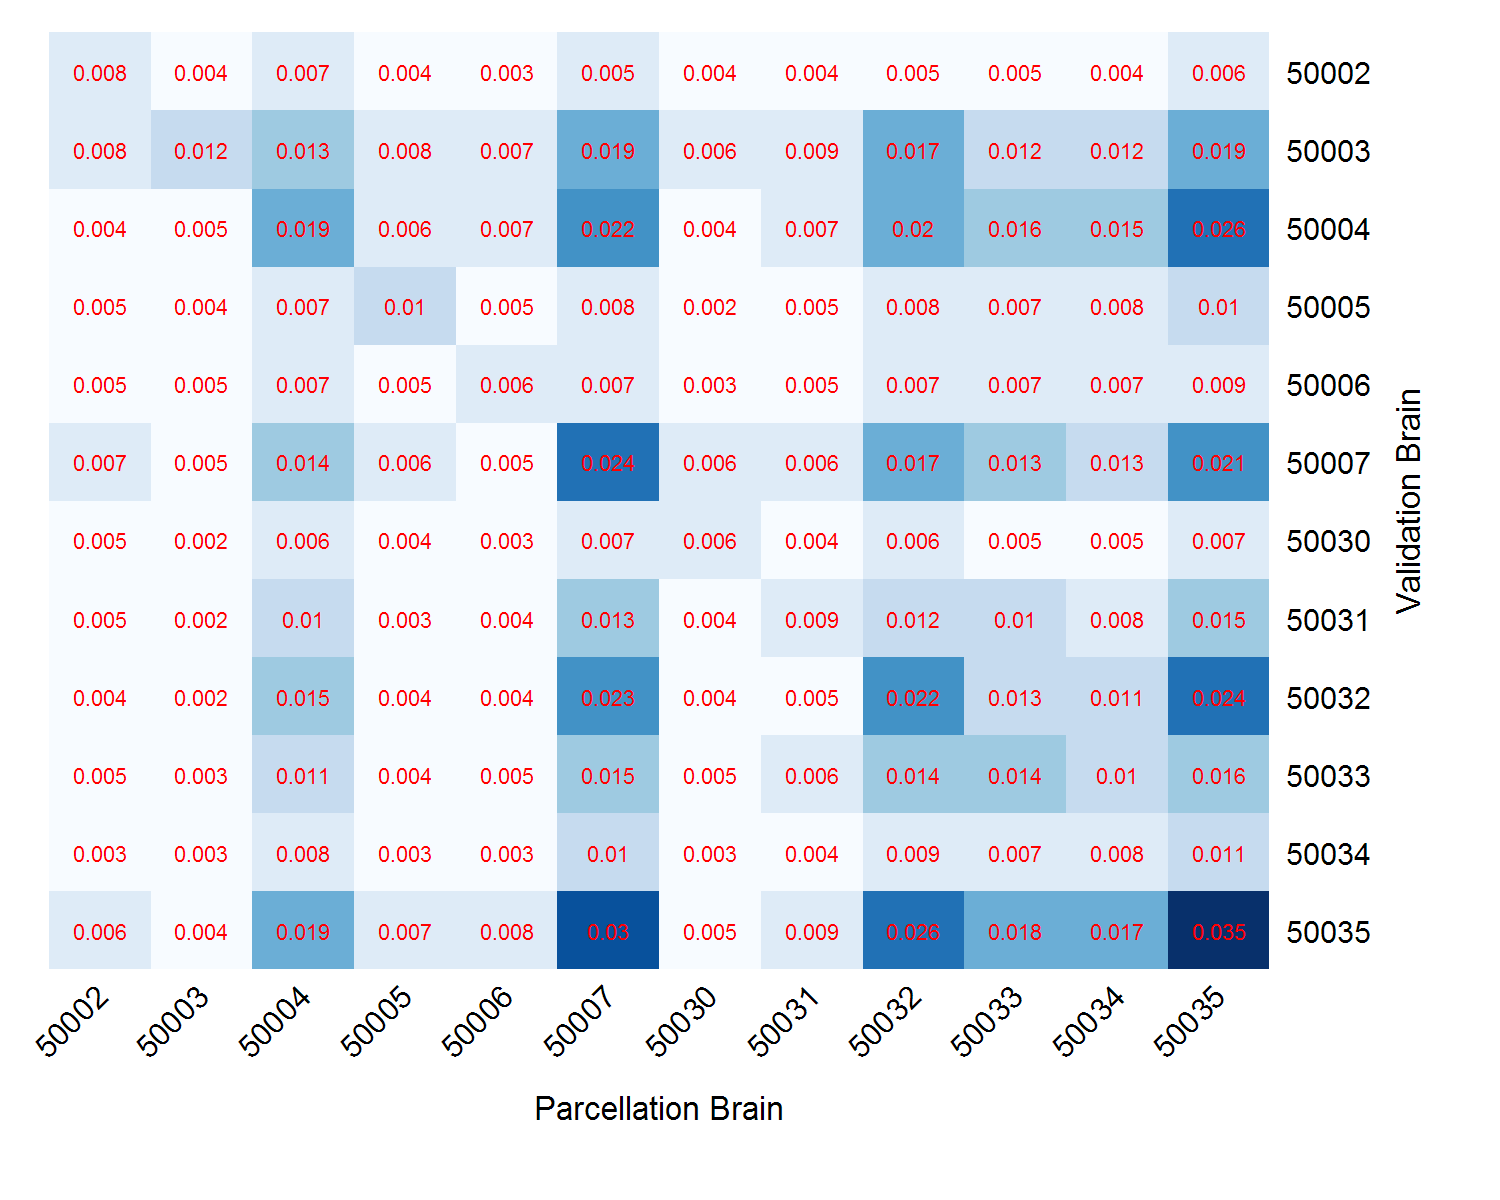
\includegraphics[scale = 1]{figs/8_cv_sp.png}
\end{figure}

Figure (\ref{cv_sp}) shows the results of the cross-validation procedure
using the spectral partitioning method.

\section{Conclusion}


{\color{red}Some things to think about: Future Work, general thoughts about
parcellation, which methods did you expect to do well and which actually did
well.}


\bibliography{ref}
\bibliographystyle{apalike}

\end{document}